

\numberwithin{equation}{section}
\numberwithin{lemma}{section}

\section{Penalty Matrix in (\ref{tractormse})}\label{PenaltyTermDetails}

The $i$-th $\Omega^{(i)}$ is a $2n \times 2n$ bandwidth four symmetric matrix and its non-zero elements on the upper triangular are 
\begin{align}
\Omega_{2i-1,2i-1}^{(i)} & =\int_{t_{i}}^{t_{i+1}} \frac{d^2 h_{00}^{(i)}(t)}{dt^2}  \frac{d^2 h_{00}^{(i)}(t)}{dt^2} dt=\frac{12}{\Delta_i^3}\\
\Omega_{2i-1,2i}^{(i)} &=\int_{t_{i}}^{t_{i+1}} \frac{d^2 h_{00}^{(i)}(t)}{dt^2}  \frac{d^2 h_{10}^{(i)}(t)}{dt^2} dt=\frac{6}{\Delta_i^2}\\
\Omega_{2i-1,2i+1}^{(i)} &=\int_{t_{i}}^{t_{i+1}} \frac{d^2 h_{00}^{(i)}(t)}{dt^2}  \frac{d^2 h_{01}^{(i+1)}(t)}{dt^2} dt=\frac{-12}{\Delta_i^3}\\
\Omega_{2i-1,2i+2}^{(i)} &=\int_{t_{i}}^{t_{i+1}} \frac{d^2 h_{00}^{(i)}(t)}{dt^2}  \frac{d^2 h_{11}^{(i+1)}(t)}{dt^2} dt=\frac{6}{\Delta_i^2}\\
\Omega_{2i,2i}^{(i)} &=\int_{t_{i}}^{t_{i+1}} \frac{d^2 h_{10}^{(i)}(t)}{dt^2}  \frac{d^2 h_{10}^{(i)}(t)}{dt^2} dt=\frac{4}{\Delta_i} \\
\Omega_{2i,2i+1}^{(i)} &=\int_{t_{i}}^{t_{i+1}} \frac{d^2 h_{10}^{(i)}(t)}{dt^2}  \frac{d^2 h_{01}^{(i+1)}(t)}{dt^2} dt=\frac{-6}{\Delta_i^2}\\
\Omega_{2i,2i+2}^{(i)} &=\int_{t_{i}}^{t_{i+1}} \frac{d^2 h_{10}^{(i)}(t)}{dt^2}  \frac{d^2 h_{11}^{(i+1)}(t)}{dt^2} dt=\frac{2}{\Delta_i}\\
\Omega_{2i+1,2i+1}^{(i)} &=\int_{t_{i}}^{t_{i+1}} \frac{d^2 h_{01}^{(i+1)}(t)}{dt^2}  \frac{d^2 h_{01}^{(i+1)}(t)}{dt^2} dt=\frac{12}{\Delta_i^3}\\
\Omega_{2i+1,2i+2}^{(i)} &=\int_{t_{i}}^{t_{i+1}} \frac{d^2 h_{01}^{(i+1)}(t)}{dt^2}  \frac{d^2 h_{11}^{(i+1)}(t)}{dt^2} dt=\frac{-6}{\Delta_i^2}\\
\Omega_{2i+2,2i+2}^{(i)} &=\int_{t_{i}}^{t_{i+1}} \frac{d^2 h_{11}^{(i+1)}(t)}{dt^2}  \frac{d^2 h_{11}^{(i+1)}(t)}{dt^2} dt=\frac{4}{\Delta_i}
\end{align}
where $\Delta_i=T_{i+1}-T_i$ and $i=1,2,\ldots,n-1$. Then 
\begin{equation*}
\mathbf{\Omega}=\sum_{i=1}^{n-1}\lambda_i\Omega^{(i)}
\end{equation*}


\section{Proof of Theorem \ref{TractorSplineTheorem}}\label{AppendixTractorSplineProof}

\begin{proof}
%The proof is based on Ex. 5.7 of \cite{esl2009}, and is essentially a proof by contradiction. If $g:[a,b]\to \mathbb{R}$ is a proposed minimizer, then we can construct a cubic spline $f(t)$ that agrees with $g(t)$ and its first derivatives at $t_1,\ldots,t_n$, and is component-wise linear on $[a, t_1]$ and $[t_n, b]$. This means the first two terms of the objective function will be the same for $f(t)$ and $g(t)$. We now show that the curvature penalty ...
If $g:[a,b]\to \mathbb{R}$ is a proposed minimizer, construct a cubic spline $f(t)$ that agrees with $g(t)$ and its first derivatives at $t_1,\ldots,t_n$, and is component-wise linear on $[a, t_1]$ and $[t_n, b]$. Let $h(t) = g(t)-f(t)$. Then, for $i = 1,\dots ,n-1$, 
\begin{align*}
\int_{t_i}^{t_{i+1}}f''(t)h''(t)dt &=f''(t)h'(t) \bigg\rvert_{t_i}^{t_{i+1}}-\int_{t_i}^{t_{i+1}}f'''(t)h'(t)dt \\
&= 0-f'''(t_i^+)\int_{t_i}^{t_{i+1}}h'(t)dt \\
&= -f'''(t_i^+)\left( h(t_{i+1}) -h(t_i) \right)\\
&=0.
\end{align*}
Additionally, $\int_{a}^{t_1}f''(t)h''(t)dt=\int_{t_n}^{b}f''(t)h''(t)dt=0$, since $f(t)$ is assumed linear outside the knots. Thus, for $i=0,\ldots,n$, 
\begin{align*}
\int_{t_i}^{t_{i+1}}\lvert g''(t) \rvert^2dt &= \int_{t_i}^{t_{i+1}}\lvert f''(t)+h''(t)\rvert^2 dt\\
&= \int_{t_i}^{t_{i+1}}\lvert f''(t)\rvert^2dt+2\int_{t_i}^{t_{i+1}}f''(t)h''(t)dt+\int_{t_i}^{t_{i+1}}\lvert h''(t)\rvert^2dt\\
&=\int_{t_i}^{t_{i+1}}\lvert f''(t)\rvert^2dt+\int_{t_i}^{t_{i+1}}\lvert h''(t)\rvert^2dt\\
&\geq \int_{t_i}^{t_{i+1}}\lvert f''(t)\rvert^2dt.
\end{align*}
The result $J[f]\leq J[g]$ follows since $\lambda_i>0$. 

Furthermore, equality of the curvature penalty term only holds if $g(t) = f(t)$. On $[t_1, t_n]$, we require $h''(t) = 0$ but since $h(ti) = h'(ti) = 0$ for $i = 1, \ldots , n$, this means $h(t) = 0$. Meanwhile on $[a, t_1]$ and $[t_n, b]$, $f''(t) = 0$ so that equality requires $g''(t)=0$. Since $f(t)$ agrees with $g(t)$ and its first derivatives at $t_1$ and $t_n$, equality is forced on both intervals.
\end{proof}

\section{Proof of Theorem \ref{basisindependent}}\label{AppendixBasisproof}

To prove Theorem \ref{basisindependent}, we are introducing a Lemma \cite{Peng1983linear} in the first place. 

\begin{lemma}\label{basiscontinuousLemma}
Functions $N_1(t),N_2(t),\ldots,N_n(t)$ on interval $[a,b]$, if they are linear dependent, the necessary and sufficient condition is for any $c_1,c_2,\ldots,c_n \in [a,b]$, the determinant $D(c_1,c_2,\ldots,c_n)=0$; if they are linear independent, the necessary and sufficient condition is that there exist $c_1,c_2,\ldots,c_n \in [a,b]$, so that the determinant $D(c_1,c_2,\cdots,c_n) \neq 0$, where 
\begin{equation*}
D(c_1,c_2,\ldots,c_n)=
\begin{vmatrix}
N_1(c_1) & N_1(c_2) & \cdots& N_1(c_n)\\
N_2(c_1) & N_2(c_2)& \cdots & N_2(c_n)\\
 \vdots  &  \vdots  & \ddots  & \vdots  \\  
N_n(c_1) & N_n(c_2) & \cdots & N_n(c_n)\\
\end{vmatrix}
\end{equation*}
\end{lemma}

In the following, we are proving Theorem \ref{basisindependent} with the help of Lemma \ref{basiscontinuousLemma}. 

\begin{proof}
It is obvious that these basis functions are continuous on subinterval $[t_i,t_{i+1}]$, where $i=1,\ldots,n-1$. We will prove that these basis functions are independent at first. 

Given $2n$ basis functions and $n$ knots, we choose $t_1, \frac{t_1+t_2}{2}, t_2, \frac{t_2+t_3}{2}, \cdots, t_{n-1}$, $\frac{t_{n-1}+t_n}{3}$, $\frac{2(t_{n-1}+t_n)}{3}, t_n$ as new $2n$ knots, and denoted by $c_1,c_2,\cdots,c_{2n}$. Then the determinant is
\begin{align}\label{matrixD}
D(c_1,c_2,\cdots,c_{2n})=&
\begin{bmatrix}
N_1(c_1) & N_1(c_2) & \cdots& N_1(c_{2n})\\
N_2(c_1) & N_2(c_2)& \cdots & N_2(c_{2n})\\
 \vdots  &  \vdots  & \ddots  & \vdots  \\  
N_{2n}(c_1) & N_{2n}(c_2) & \cdots & N_{2n}(c_{2n})\\
\end{bmatrix}
\end{align}
%where $D(c_1,c_2,\cdots,c_{2n})=\begin{cases}
%N_1(t_1)=1 \\
%N_1(\frac{t_1+t_2}{2})=a_{12} \\
%N_2(t_1)=0 \\
%N_2(\frac{t_1+t_2}{2})=a_{22} \\
%N_{2i+1}(\frac{t_i+t_{i+1}}{2})=a_{2i+1,2i} \\ 
%N_{2i+1}(t_{i+1})=1  \\ 
%N_{2i+1}(\frac{t_{i+1}+t_{i+2}}{2})=a_{2i+1,2i+2}  \\ 
%N_{2i+2}(\frac{t_i+t_{i+1}}{2})=a_{2i+2,2i} \\ 
%N_{2i+2}(\frac{t_{i+1}+t_{i+2}}{2})=a_{2i+2,2i+2} \\ 
%N_{2n-1}(t_{2n-1})=0 \\
%N_{2n-1}(\frac{t_{2n-1}+t_{2n}}{3})=a_{2n-1,2n-2} \\
%N_{2n-1}(\frac{2(t_{2n-1}+t_{2n})}{3})=a_{2n-1,2n-1} \\
%N_{2n-1}(t_{2n})=1 \\
%N_{2n}(\frac{t_{2n-1}+t_{2n}}{3})=a_{2n,2n-2} \\
%N_{2n}(\frac{2(t_{2n-1}+t_{2n})}{3})=a_{2n,2n-1} \\
%N_{2n}(t_{2n})=0 \\
%0 &  \mbox{otherwise}
%\end{cases}$,\\
where the non-zero elements of matrix $D$ are \begin{align*}
\begin{matrix}
N_1(t_1)=1 & N_1\left(\frac{t_1+t_2}{2}\right)=a_{12} &  N_2(t_1)=0 \\ N_2\left(\frac{t_1+t_2}{2}\right)=a_{22} & N_{2i+1}\left(\frac{t_i+t_{i+1}}{2}\right)=a_{2i+1,2i} & N_{2i+1}(t_{i+1})=1  \\ 
N_{2i+1}\left(\frac{t_{i+1}+t_{i+2}}{2}\right)=a_{2i+1,2i+2}  & 
N_{2i+2}\left(\frac{t_i+t_{i+1}}{2}\right)=a_{2i+2,2i} &
N_{2i+2}\left(\frac{t_{i+1}+t_{i+2}}{2}\right)=a_{2i+2,2i+2} \\
 N_{2n-1}(t_{2n-1})=0 & N_{2n-1}\left(\frac{t_{2n-1}+t_{2n}}{3}\right)=a_{2n-1,2n-2} &
N_{2n-1}\left(\frac{2(t_{2n-1}+t_{2n})}{3}\right)=a_{2n-1,2n-1} \\
N_{2n-1}(t_{2n})=1 & N_{2n}(\frac{t_{2n-1}+t_{2n}}{3})=a_{2n,2n-2} &
N_{2n}\left(\frac{2(t_{2n-1}+t_{2n})}{3}\right)=a_{2n,2n-1} \\
N_{2n}(t_{2n})=0 
\end{matrix}
\end{align*}
where $i=1,\ldots,n-1$. By decomposing determinant $D$ in the following way, it will give us 
\begin{align*}
\det D= & 
\begin{vmatrix}
1 & a_{12} & 0 & 0 & \cdots& 0 & 0 \\
0 & a_{22} & 0 & 0 & \cdots& 0 & 0\\
0 & a_{32} & 1 & a_{34} & \cdots& 0 & 0\\
 \vdots  &  \vdots  &  \vdots &  \vdots & \ddots  & \vdots   &  \vdots\\  
0 & 0 & 0 & 0 & \cdots& a_{2n-1,2n-1} & 1\\
0 & 0 & 0 & 0 & \cdots& a_{2n,2n-1} & 0 \\
\end{vmatrix} =
\begin{vmatrix}
 a_{22} & 0 & 0 & \cdots& 0 & 0\\
 a_{32} & 1 & a_{34} & \cdots& 0 & 0\\
  \vdots  &  \vdots &  \vdots & \ddots  & \vdots   &  \vdots\\  
0 & 0 & 0 & \cdots& a_{2n-1,2n-1} & 1\\
0 & 0 & 0 & \cdots& a_{2n,2n-1} & 0 \\
\end{vmatrix} 
\\ &=a_{22}
\begin{vmatrix}
 1 & a_{34} & \cdots& 0 & 0\\
  \vdots &  \vdots & \ddots  & \vdots   &  \vdots\\  
 0 & 0 & \cdots& a_{2n-1,2n-1} & 1\\
 0 & 0 & \cdots& a_{2n,2n-1} & 0 \\
\end{vmatrix}
\cdots =a_{22}a_{44}\cdots a_{2n-4,2n-4} 
\begin{vmatrix}
a_{2n-2,2n-2} & a_{2n-2,2n-1}  & 0\\
a_{2n-1,2n-2} & a_{2n-1,2n-1} & 1\\
 a_{2n,2n-2} &  a_{2n,2n-1} & 0 \\
\end{vmatrix}\\
=& a_{22}a_{44}\cdots a_{2n-4,2n-4} (a_{2n-2,2n-1}a_{2n,2n-2}-a_{2n,2n-1}a_{2n-2,2n-2}) \neq 0.
\end{align*}
With the conclusion of Lemma \ref{basiscontinuousLemma}, $N_1(t),\ldots,N_{2n}(t)$  are linearly independent on interval $[t_1, t_n]$.

Secondly, we will prove that basis functions represent any cubic function on each interval $[t_i, t_{i+1}]$. Due to the definition of cubic spline, on interval $[t_i, t_{i+1}]$, a cubic spline $g(t)$ can be written in the form of
\begin{eqnarray}
g(t)=d_i (t-t_i)^3+c_i(t-t_i)^2+b_i(t-t_i)+a_i, \mbox{for $t_i \leq t \leq t_{i+1}$}
\end{eqnarray}
For any $f(t)$ on $[t_1, t_n]$, it can be represented as $f(t)=\sum_{k=1}^{2n} \theta_k N_k(t)$. Then for $\forall t \in [t_i,t_{i+1}]$, $i=1,\ldots,n-1$, we have
\begin{align*}
f(t)=\begin{cases}
\theta_{2i-1}N_{2i-1}(t)+\theta_{2i}N_{2i}(t)+\theta_{2i+1}N_{2i+1}(t)+\theta_{2i+2}N_{2i+3}(t), & t_i \leq t \leq t_{i+1}  \\
0, & \mbox{otherwise}\\
\end{cases}
\end{align*}
Hence, 
\begin{align*}
f(t)=&\theta_{2i-1}\left( 2\left(\frac{t-t_{i}}{t_{i+1}-t_{i}}\right)^3-3\left(\frac{t-t_{i}}{t_{i+1}-t_{i}}\right)^2+1  \right) +\theta_{2i} \left( \frac{(t-t_{i})^3}{(t_{i+1}-t_{i})^2}-2\frac{(t-t_{i})^2}{t_{i+1}-t_{i}}+(t-t_{i}) \right) \\
+&\theta_{2i+1} \left( -2\left(\frac{t-t_i}{t_{i+1}-t_i}\right)^3+3\left(\frac{t-t_i}{t_{i+1}-t_i}\right)^2 \right)  +\theta_{2i+2} \left( \frac{(t-t_i)^3}{(t_{i+1}-t_i)^2}-\frac{(t-t_i)^2}{t_{i+1}-t_i} \right).
\end{align*}
After rearranging, we have
\begin{align*}
f(t)=& \left(\frac{2\theta_{2i-1}}{(t_{i+1}-t_{i})^3} +\frac{\theta_{2i}}{(t_{i+1}-t_{i})^2} -\frac{2\theta_{2i+1}}{(t_{i+1}-t_{i})^3} +\frac{\theta_{2i+2}}{(t_{i+1}-t_{i})^2} \right)  (t-t_i)^3 \\
+& \left(-\frac{3\theta_{2i-1}}{(t_{i+1}-t_{i})^2} -\frac{2\theta_{2i}}{(t_{i+1}-t_{i})} +\frac{3\theta_{2i+1}}{(t_{i+1}-t_{i})^2} - \frac{\theta_{2i+2}}{(t_{i+1}-t_{i})}\right)  (t-t_i)^2 \\
+&  \theta_{2i} (t-t_i) +\theta_{2i-1},
\end{align*}
where coefficients are
\begin{align*}
\begin{cases}
\theta_{2i-1}=a_i\\
\theta_{2i}=b_i\\
-\frac{3\theta_{2i-1}}{(t_{i+1}-t_{i})^2} -\frac{2\theta_{2i}}{(t_{i+1}-t_{i})} +\frac{3\theta_{2i+1}}{(t_{i+1}-t_{i})^2} - \frac{\theta_{2i+2}}{(t_{i+1}-t_{i})}=c_i\\
\frac{2\theta_{2i-1}}{(t_{i+1}-t_{i})^3} +\frac{\theta_{2i}}{(t_{i+1}-t_{i})^2} -\frac{2\theta_{2i+1}}{(t_{i+1}-t_{i})^3} +\frac{\theta_{2i+2}}{(t_{i+1}-t_{i})^2}=d_i
\end{cases}
\end{align*}
The resulting can always be solved for $\theta_{2i-1}, \theta_{2i},\theta_{2i+1},\theta_{2i+2}$ in terms of $a_i,b_i,c_i,d_i$ on interval $[t_i, t_{i+1}]$. So cubic spline on each interval can be represented by basis functions. \\

Finally, we will prove basis functions are continuous on $[t_1, t_n]$. For any knot $t_i$, where $t_1< t_i <t_n$, it is known that $f(t_i)=\theta_{2i-1}$. Moreover, 
\begin{align*}
\lim\limits_{t\rightarrow t_i+} f(t) = \lim\limits_{t\rightarrow t_i+} (\theta_{2i-1}N_{2i-1}(t)+\theta_{2i}N_{2i}(t)+\theta_{2i+1}N_{2i+1}(t)+\theta_{2i+2}N_{2i+3}(t))=\theta_{2i-1},\\
\lim\limits_{t\rightarrow t_i-} f(t) = \lim\limits_{t\rightarrow t_i-} (\theta_{2i-1}N_{2i-1}(t)+\theta_{2i}N_{2i}(t)+\theta_{2i+1}N_{2i+1}(t)+\theta_{2i+2}N_{2i+3}(t))=\theta_{2i-1}.
\end{align*}
As a result, 
\begin{align*}
\lim\limits_{t\rightarrow t_i^+} f(t) =\lim\limits_{t\rightarrow t_i^-} f(t) =f(t),
\end{align*}
$f(t)$ is continuous at knots, and then continuous on whole interval $[t_1,t_n]$.

Consequently, $f(t)$ is a continuous cubic spline on interval $[t_1,t_n]$, then $f(t)$ has continuous first and second derivatives.
\end{proof}


\section{Proof of Lemma \ref{cvlemma}}
\begin{proof}
For any spline $f$, 
\begin{equation}
\begin{split}
&\sum_{j=1}^{n}\left(y_j^*-f(t_j)\right)^2+\gamma \sum_{j=1}^{n}\left(v_j^*-f'(t_j)\right)^2+\lambda\int f''^2 \\
\geq&\sum_{j\neq i}^{n}\left(y_j^*-f(t_j)\right)^2+\gamma  \sum_{j\neq i}^{n}\left(v_j^*-f'(t_j)\right)^2+\lambda\int f''^2\\
\geq&\sum_{j\neq i}^{n}\left(y_j^*-\hat{f}^{(-i)}(t_j)\right)^2+\gamma  \sum_{j\neq i}^{n}\left(v_j^*-\hat{f}'^{(-i)}(t_j)\right)^2+\lambda\int \hat{f}^{(-i)''2}\\
=&\sum_{j=1}^{n}\left(y_j^*-\hat{f}^{(-i)}(t_j)\right)^2+\gamma  \sum_{j=1}^{n}\left(v_j^*-\hat{f}'^{(-i)}(t_j)\right)^2+\lambda\int \hat{f}^{(-i)''2}
\end{split}
\end{equation}
by the definition of $\hat{f}^{(-i)}$, $\hat{f}'^{(-i)}$ and the fact that $y_i^*=\hat{f}^{(-i)}(t_i)$, $v_i^*=\hat{f}'^{(-i)}(t_i)$. It follows that $\hat{f}^{(-i)}$ is the minimizer of the RSS function (\ref{tractorsplineObjective}), so that
\begin{align}
\mathbf{\hat{f}}^{(-i)}&=S\mathbf{y}^*+\gamma T\mathbf{v}^*\\
\mathbf{\hat{f}}'^{(-i)}&=U\mathbf{y}^*+\gamma V\mathbf{v}^*
\end{align}
\end{proof}


\section{Proof of Theorem \ref{tractorsplinecvscore}}

\begin{proof}
\begin{equation}\label{th3proofeq1}
\begin{split}
\hat{f}^{(-i)}(t_i)-y_i=& \sum_{j=1}^{n}S_{ij}y_j^*+ \gamma \sum_{j=1}^{n}T_{ij}v_j^*-y_i^*\\
=&\sum_{j\neq i}^{n}S_{ij}y_j+ \gamma \sum_{j\neq i}^{n}T_{ij}v_j+S_{ii}\hat{f}^{(-i)}(t_i)+\gamma T_{ii}\hat{f}'^{(-i)}(t_i)-y_i\\
=&\sum_{j=1}^{n}S_{ij}y_j+ \gamma \sum_{j=1}^{n}T_{ij}v_j+S_{ii}(\hat{f}^{(-i)}(t_i)-y_i)+\gamma T_{ii}(\hat{f}'^{(-i)}(t_i)-v_i)-y_i\\
=&(\hat{f}(t_i)-y_i)+S_{ii}(\hat{f}^{(-i)}(t_i)-y_i)+\gamma T_{ii}(\hat{f}'^{(-i)}(t_i)-v_i).
\end{split}
\end{equation}
Additionally, 
\begin{equation}
\begin{split}
\hat{f}'^{(-i)}(t_i)-v_i=& \sum_{j=1}^{n}U_{ij}y_j^*+ \gamma \sum_{j=1}^{n}V_{ij}v_j^*-v_i^*\\
=&\sum_{j\neq i}^{n}U_{ij}y_j+ \gamma \sum_{j\neq i}^{n}V_{ij}v_j+U_{ii}\hat{f}^{(-i)}(t_i)+\gamma V_{ii}\hat{f}'^{(-i)}(t_i)-v_i\\
=&\sum_{j=1}^{n}U_{ij}y_j+ \gamma \sum_{j=1}^{n}V_{ij}v_j+U_{ii}(\hat{f}^{(-i)}(t_i)-y_i)+\gamma V_{ii}(\hat{f}'^{(-i)}(t_i)-v_i)-v_i\\
=&(\hat{f}'(t_i)-v_i)+U_{ii}(\hat{f}^{(-i)}(t_i)-y_i)+\gamma V_{ii}(\hat{f}'^{(-i)}(t_i)-v_i).
\end{split}
\end{equation}
Therefore, 
\begin{equation}\label{th3proofeq2}
\hat{f}'^{(-i)}(t_i)-v_i = \frac{\hat{f}'(t_i)-v_i}{1-\gamma V_{ii}}+ \frac{U_{ii}(\hat{f}^{(-i)}(t_i)-y_i)}{1-\gamma V_{ii}}.
\end{equation}
After substituting equation (\ref{th3proofeq2}) into (\ref{th3proofeq1}), we get
\begin{equation}
\hat{f}^{(-i)}(t_i)-y_i=\frac{\hat{f}(t_i)-y_i+\gamma \frac{T_{ii}}{1-\gamma V_{ii}}(\hat{f}'(t_i)-v_i)}{1-S_{ii}-\gamma\frac{T_{ii}}{1-\gamma V_{ii}}U_{ii}}.
\end{equation}
As a result, 
\begin{equation}
\mbox{CV}(\lambda,\gamma)=\frac{1}{n}\sum_{i=1}^{n}\frac{\hat{f}(t_i)-y_i+\gamma \frac{T_{ii}}{1-\gamma V_{ii}}(\hat{f}'(t_i)-v_i)}{1-S_{ii}-\gamma\frac{T_{ii}}{1-\gamma V_{ii}}U_{ii}}.
\end{equation}
\end{proof}


%\clearpage

\section{Residuals Analysis}
\begin{figure}[!ht]
    \centering
    \begin{subfigure}{0.45\textwidth}
    \centering
    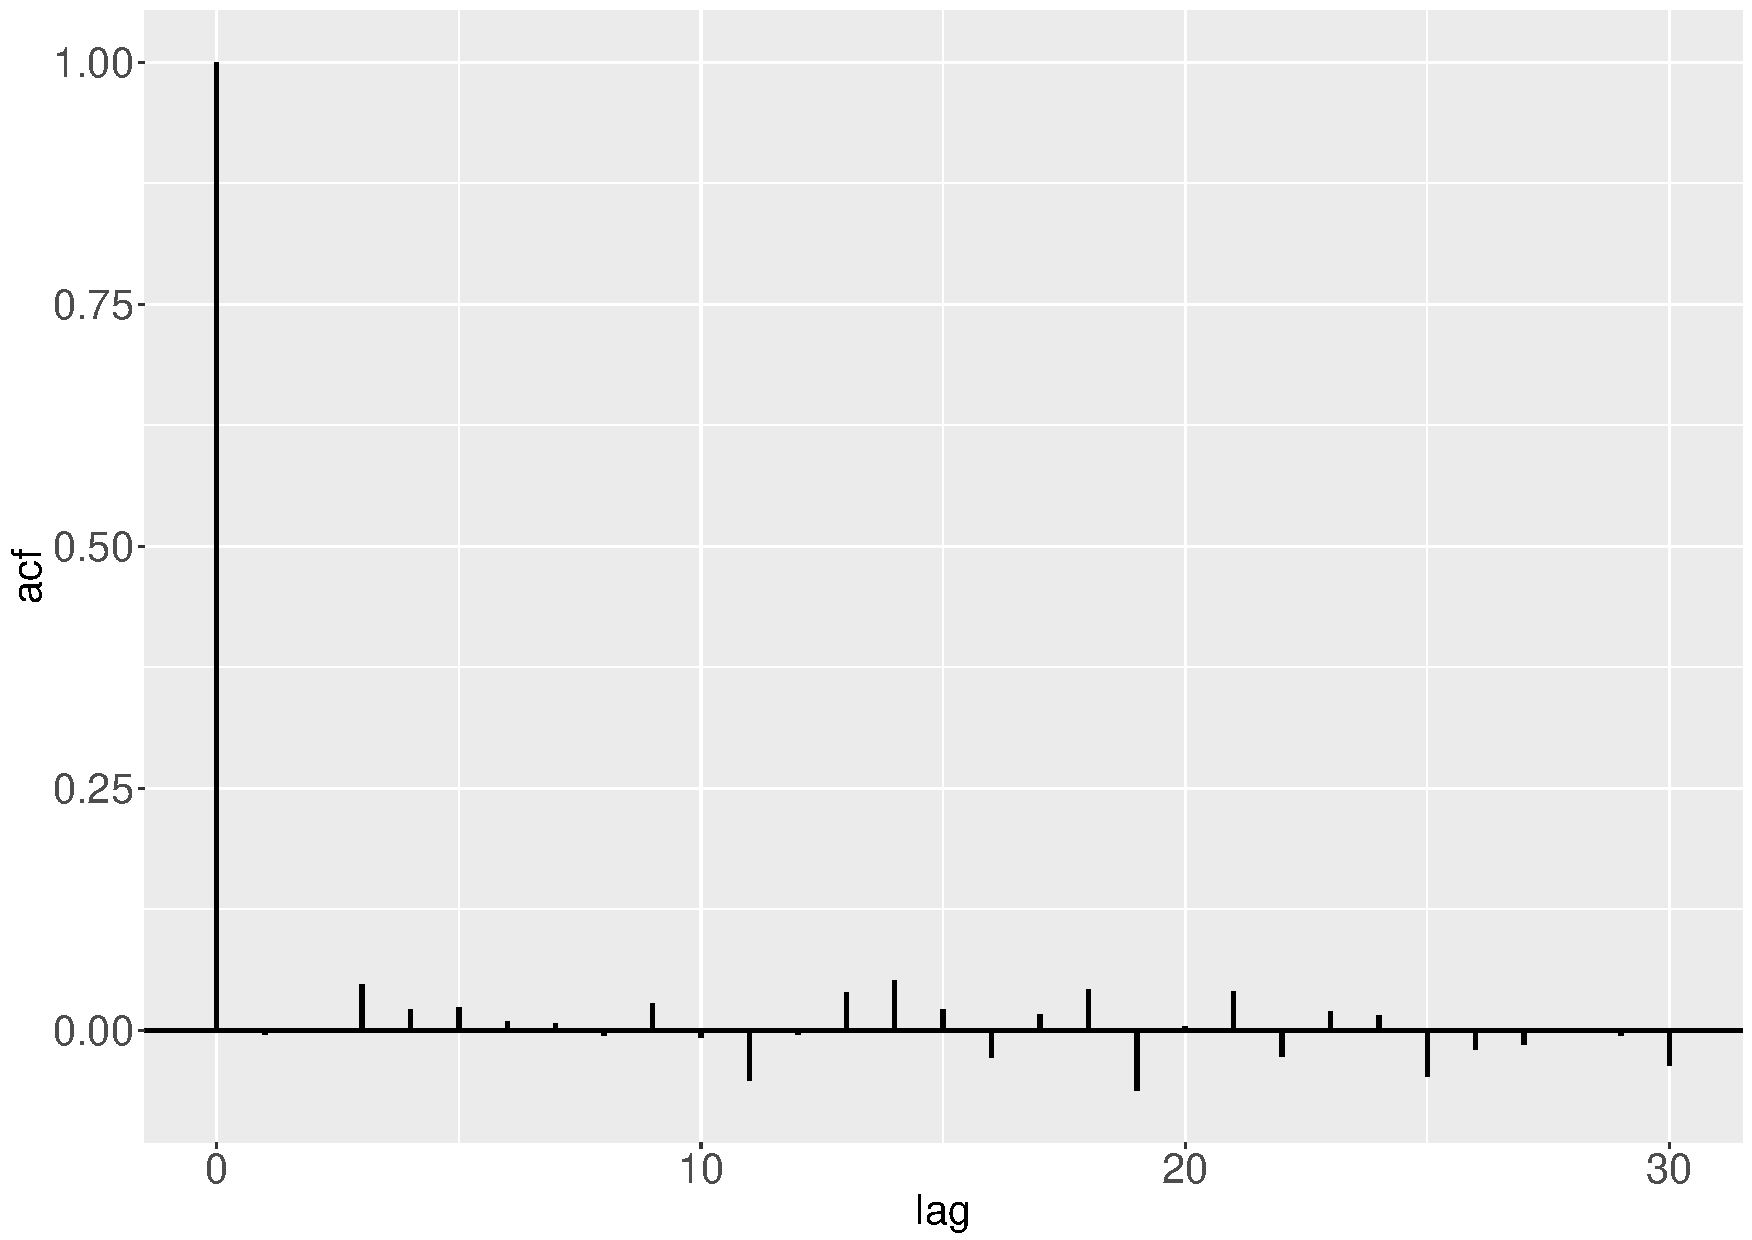
\includegraphics[width=\textwidth]{Chapters/02TractorSplineTheory/plot/ggplot/ggacfBlocks7.pdf}
    \caption{ACF of residuals from \textit{Blocks} with SNR at 7 }
    \end{subfigure}%
    \begin{subfigure}{0.45\textwidth}
    \centering
    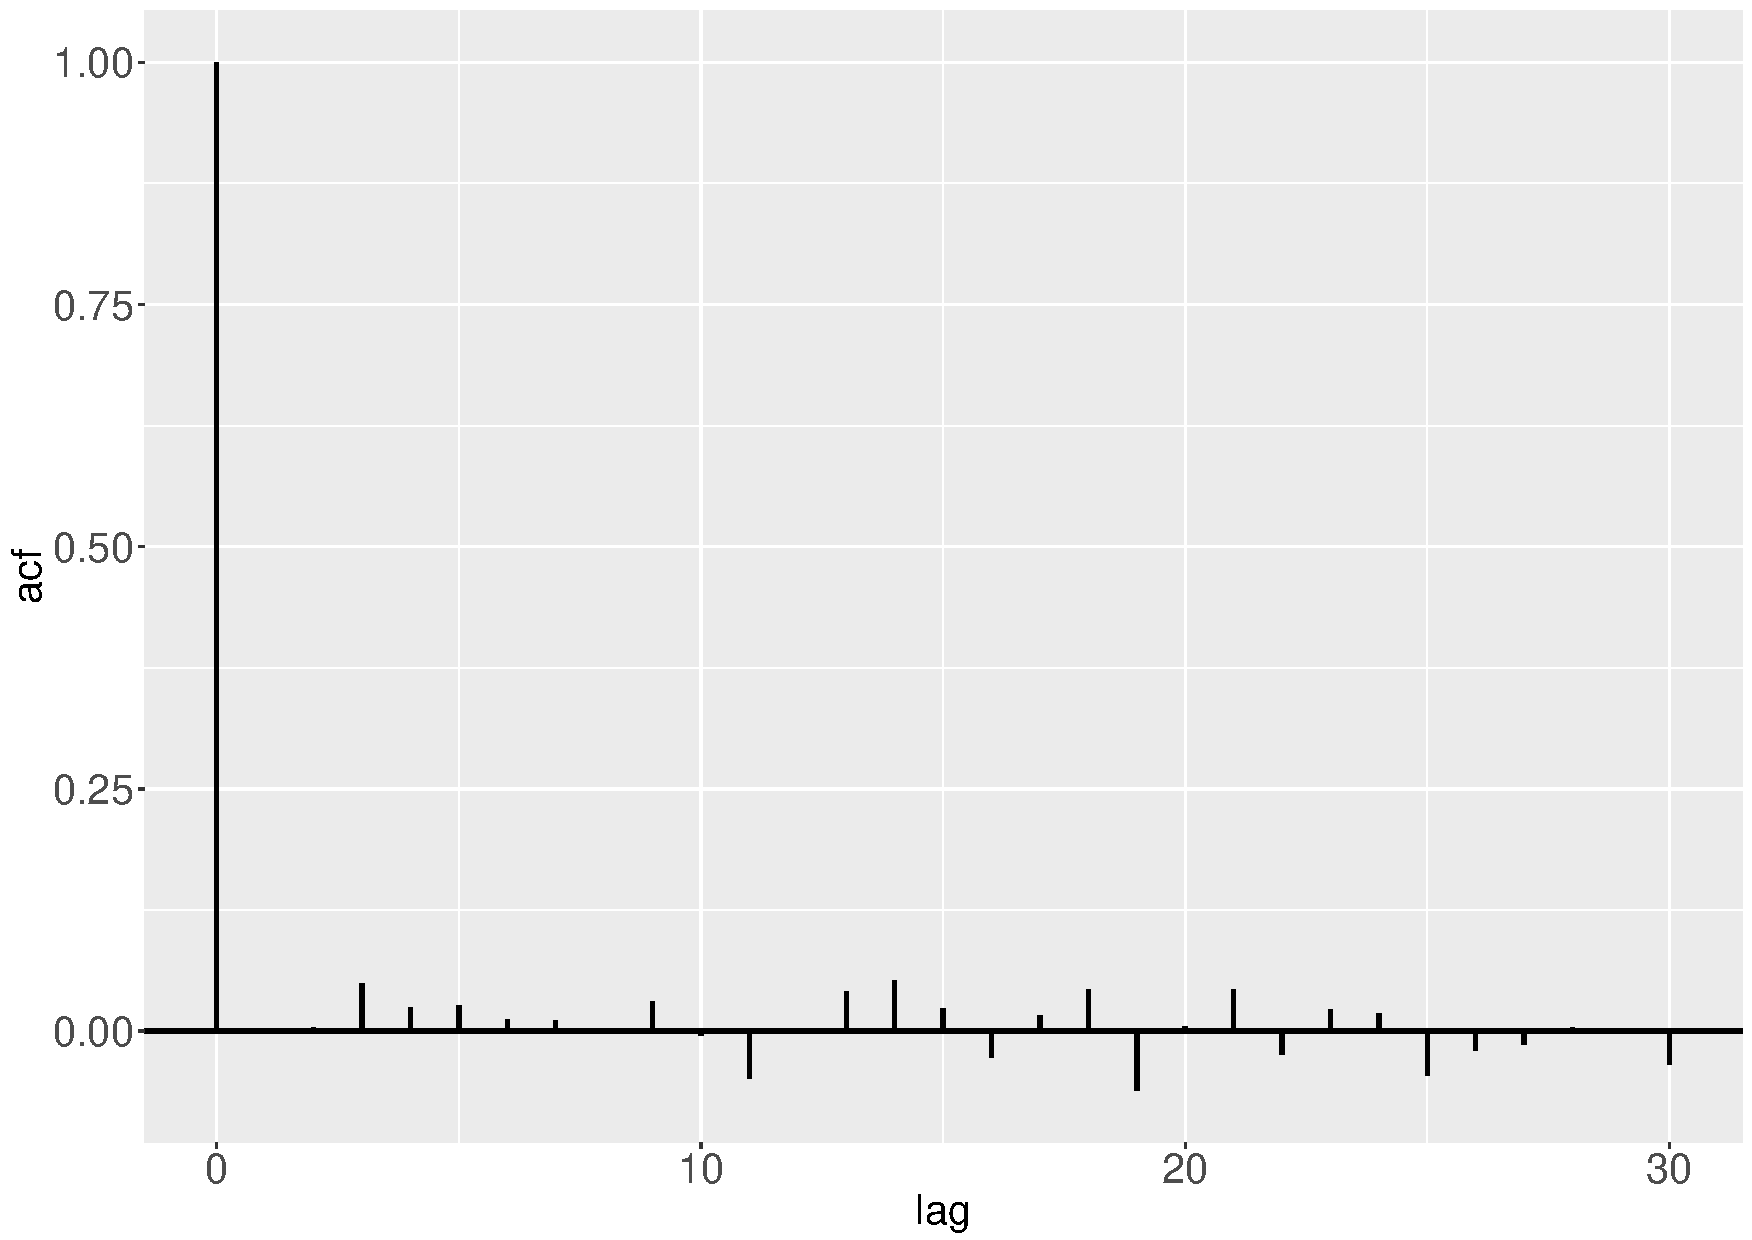
\includegraphics[width=\textwidth]{Chapters/02TractorSplineTheory/plot/ggplot/ggacfBumps7.pdf}
    \caption{ACF of residuals from \textit{Bumps} with SNR at 7 }
    \end{subfigure}
    \begin{subfigure}{0.45\textwidth}
    \centering
    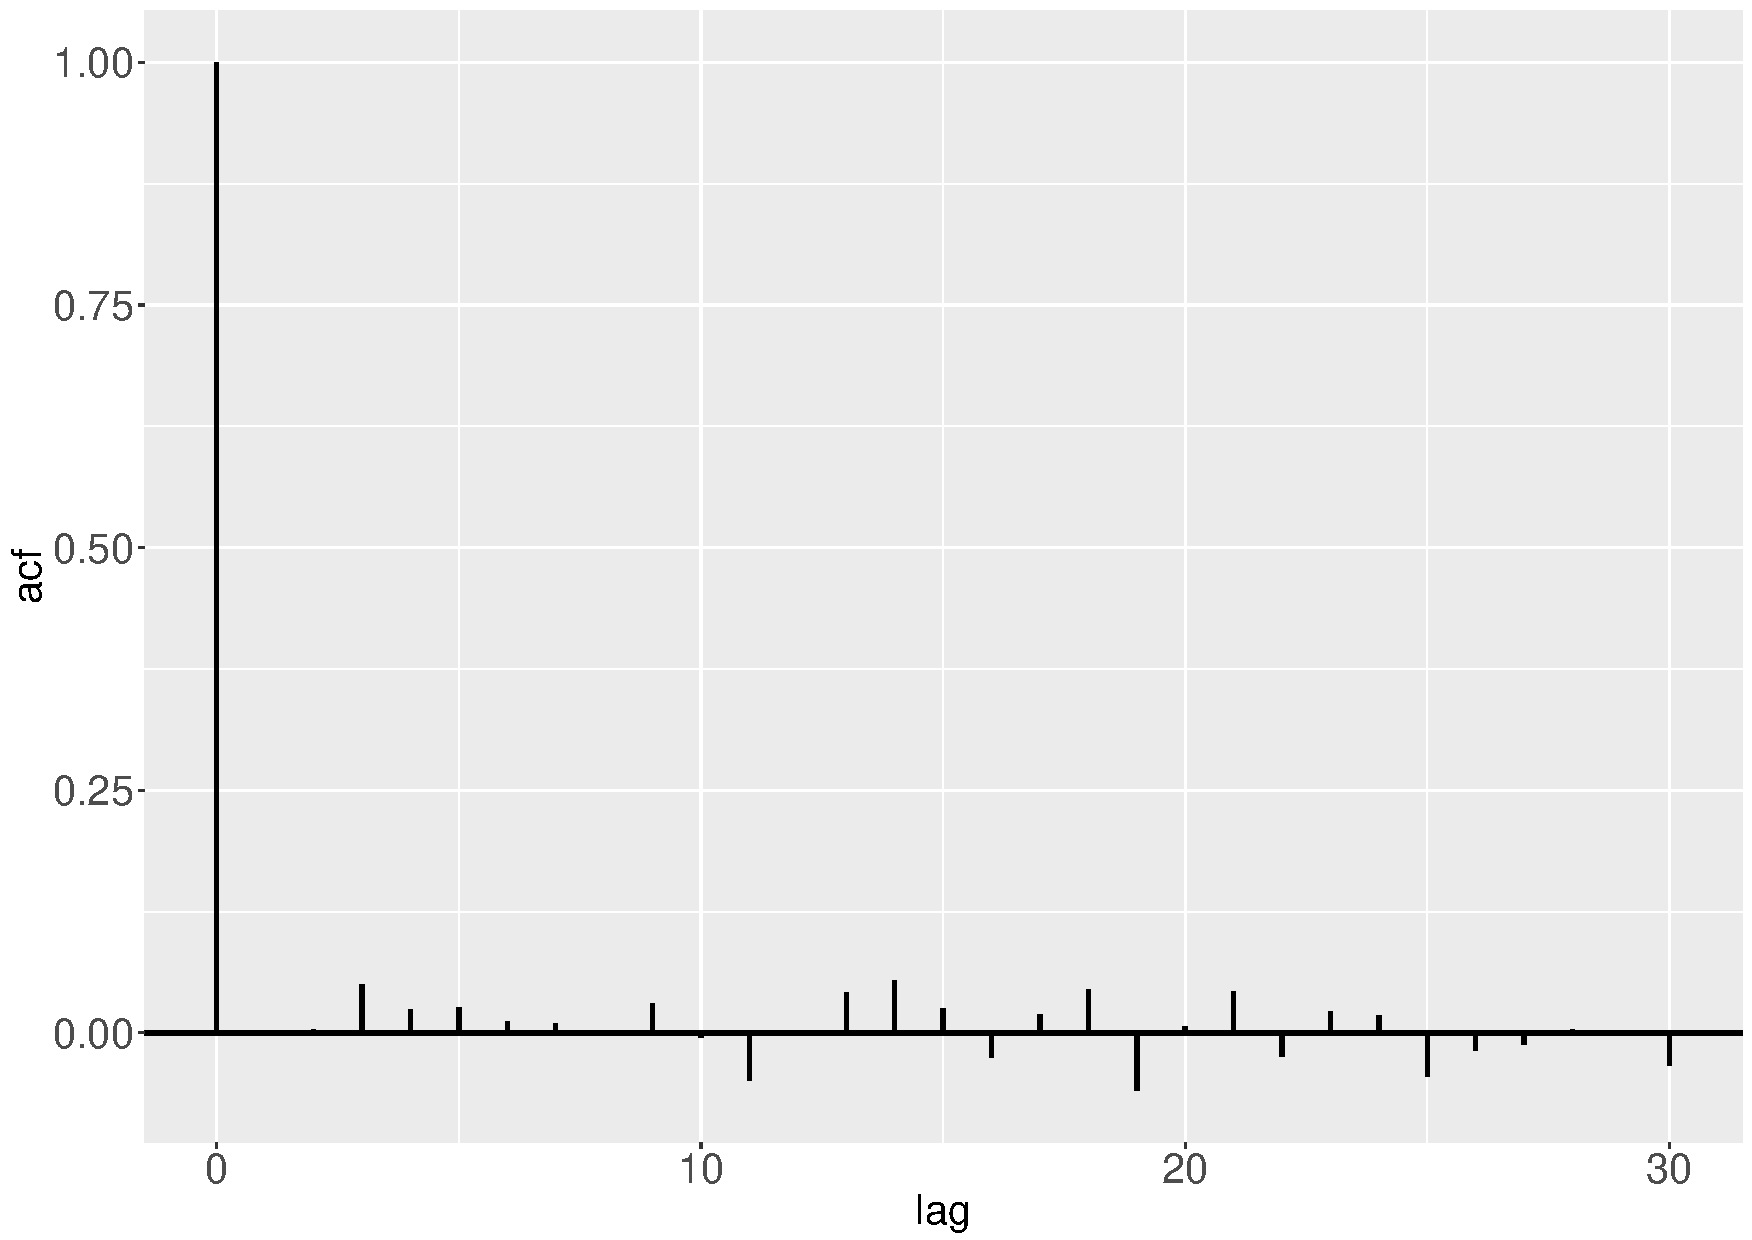
\includegraphics[width=\textwidth]{Chapters/02TractorSplineTheory/plot/ggplot/ggacfHeavi7.pdf}
    \caption{ACF of residuals from \textit{HeaviSine} with SNR at 7 }
    \end{subfigure}
    \begin{subfigure}{0.45\textwidth}
    \centering
    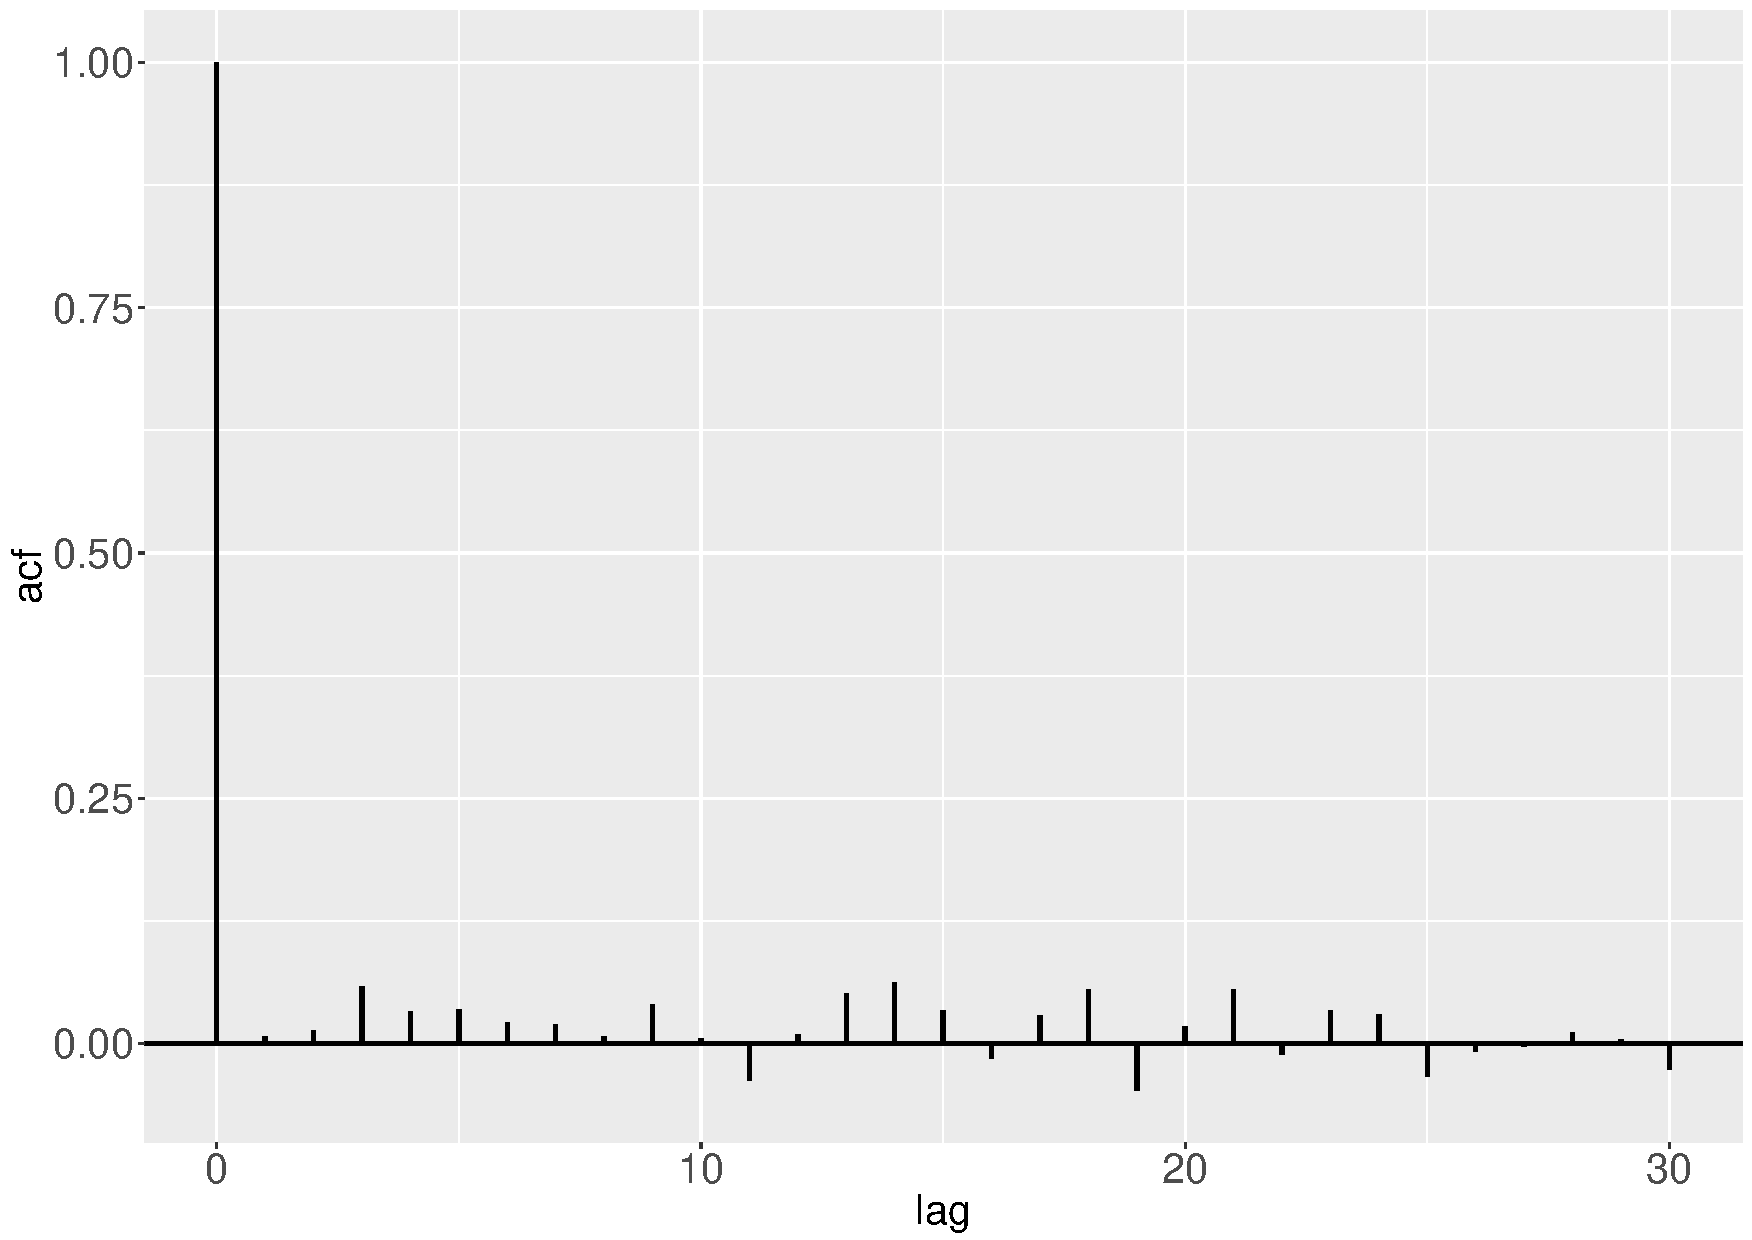
\includegraphics[width=\textwidth]{Chapters/02TractorSplineTheory/plot/ggplot/ggacfDoppler7.pdf}
    \caption{ACF of residuals from \textit{Doppler} with SNR at 7 }
    \end{subfigure}
\caption{ACF of residuals at SNR level of 7.}\label{tractorsplineSNR7acf}
 \end{figure}
\begin{figure}[!ht]
    \centering
    \begin{subfigure}{0.45\textwidth}
    \centering
    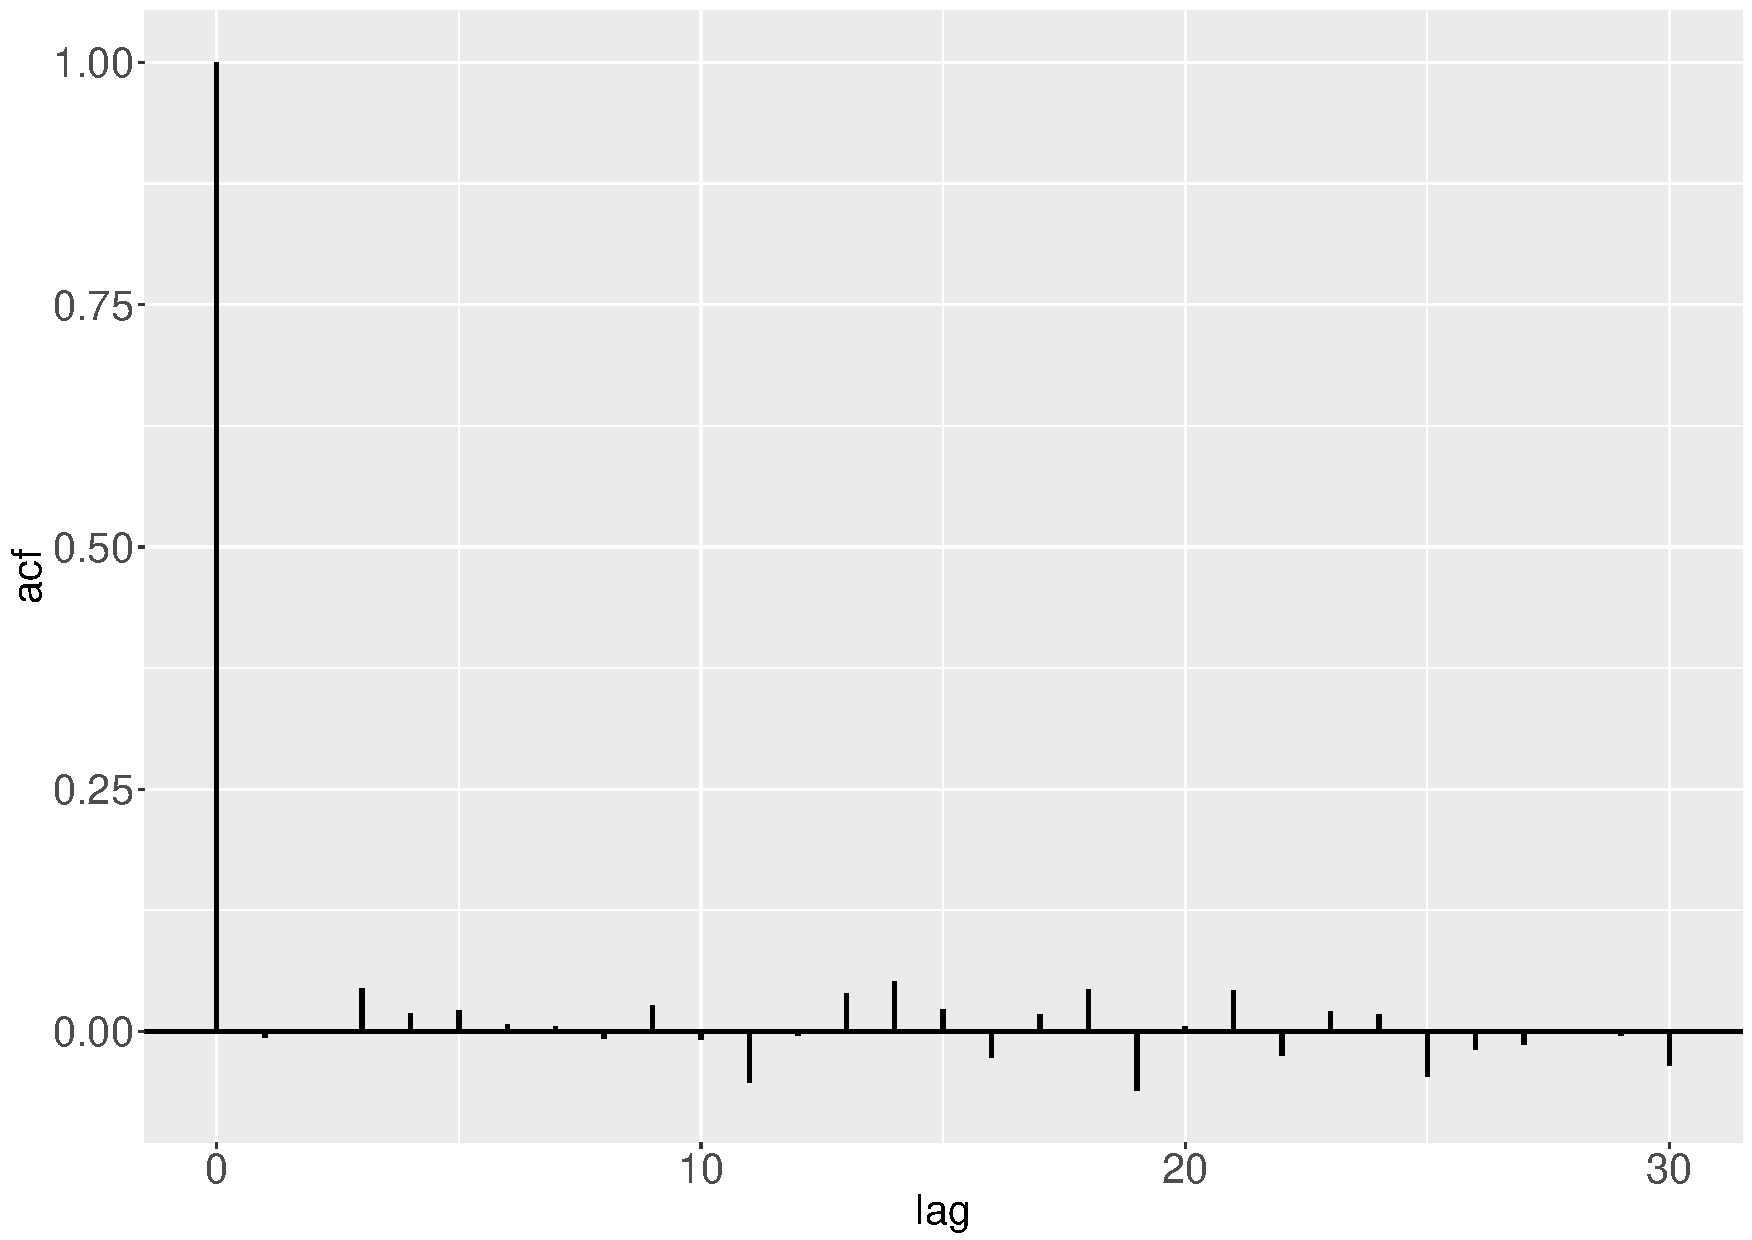
\includegraphics[width=\textwidth]{Chapters/02TractorSplineTheory/plot/ggplot/ggacfBlocks3.pdf}
    \caption{ACF of residuals from \textit{Blocks} with SNR at 3 }
    \end{subfigure}%
    \begin{subfigure}{0.45\textwidth}
    \centering
    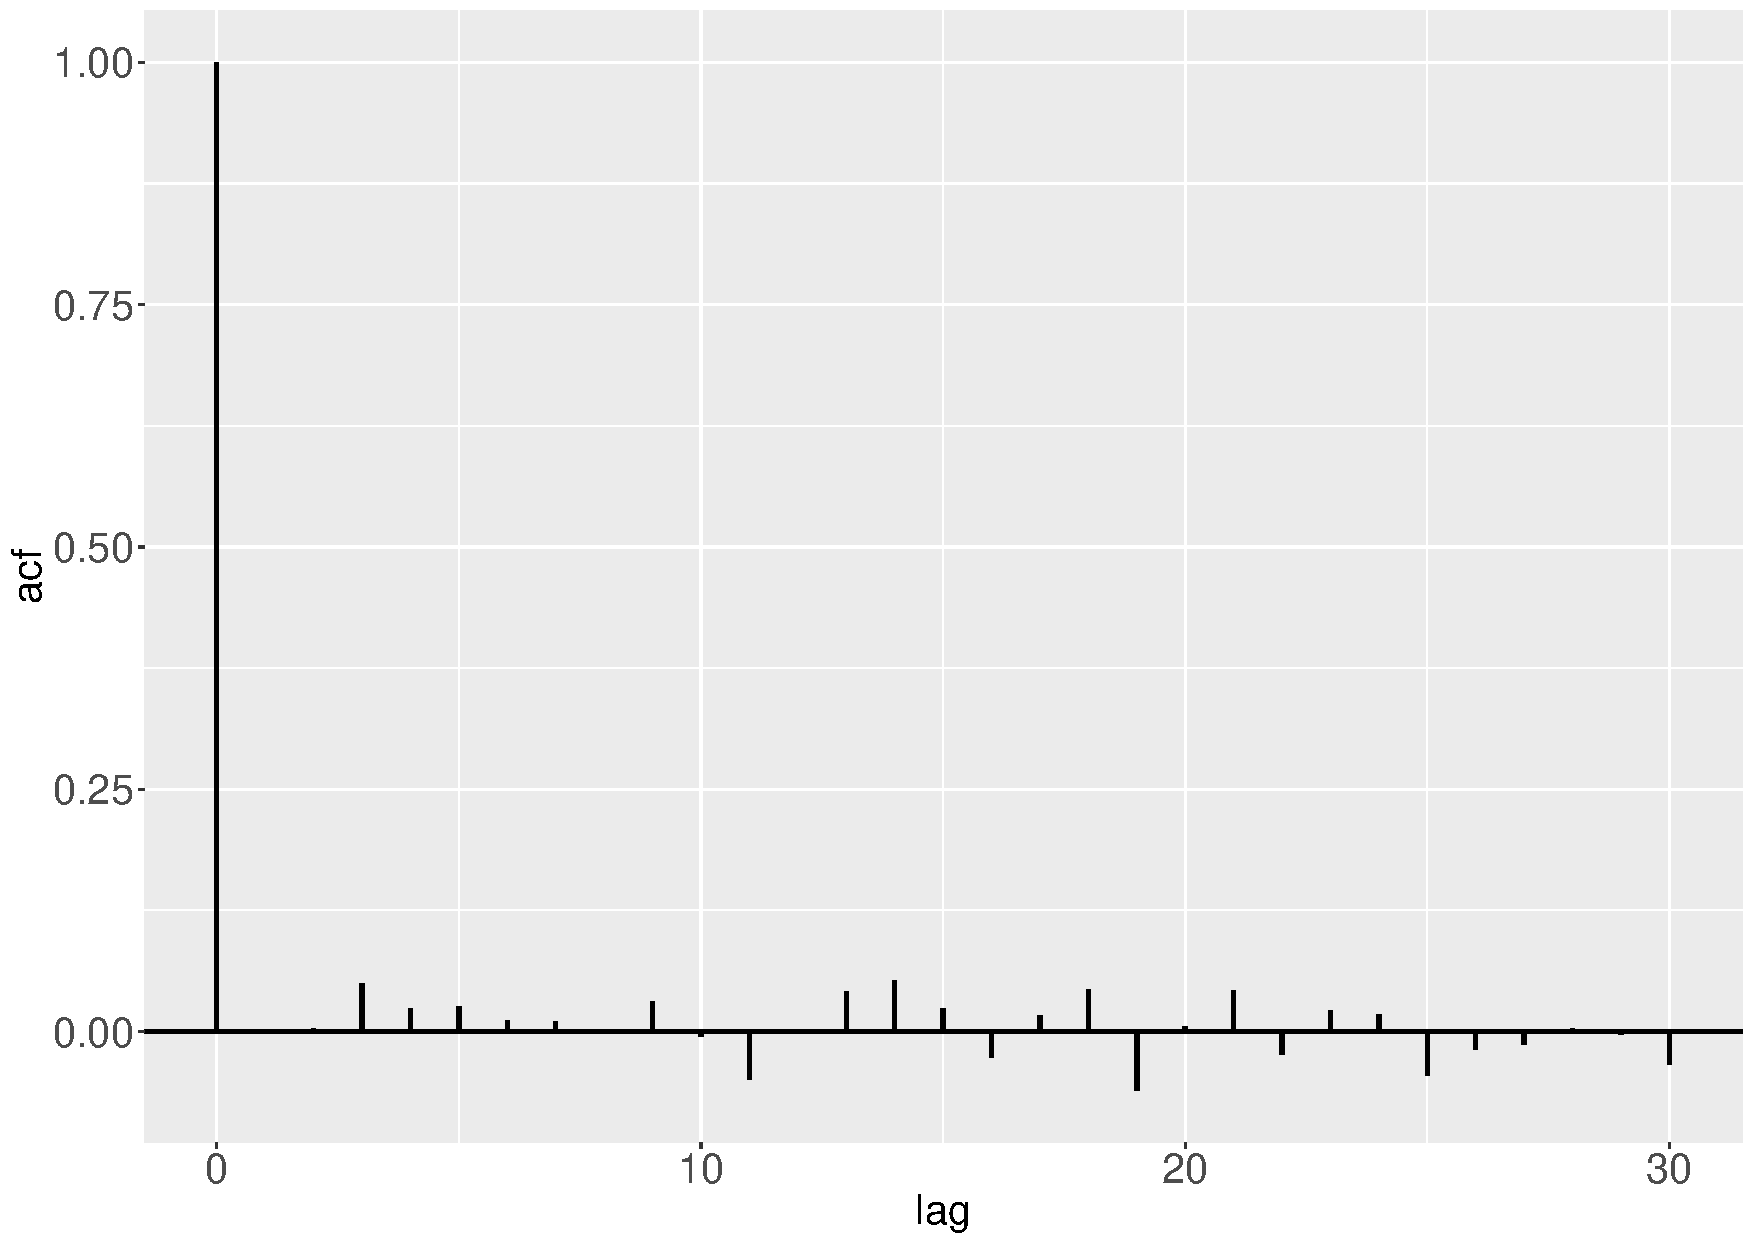
\includegraphics[width=\textwidth]{Chapters/02TractorSplineTheory/plot/ggplot/ggacfBumps3.pdf}
    \caption{ACF of residuals from \textit{Bumps} with SNR at 3 }
    \end{subfigure}
    \begin{subfigure}{0.45\textwidth}
    \centering
    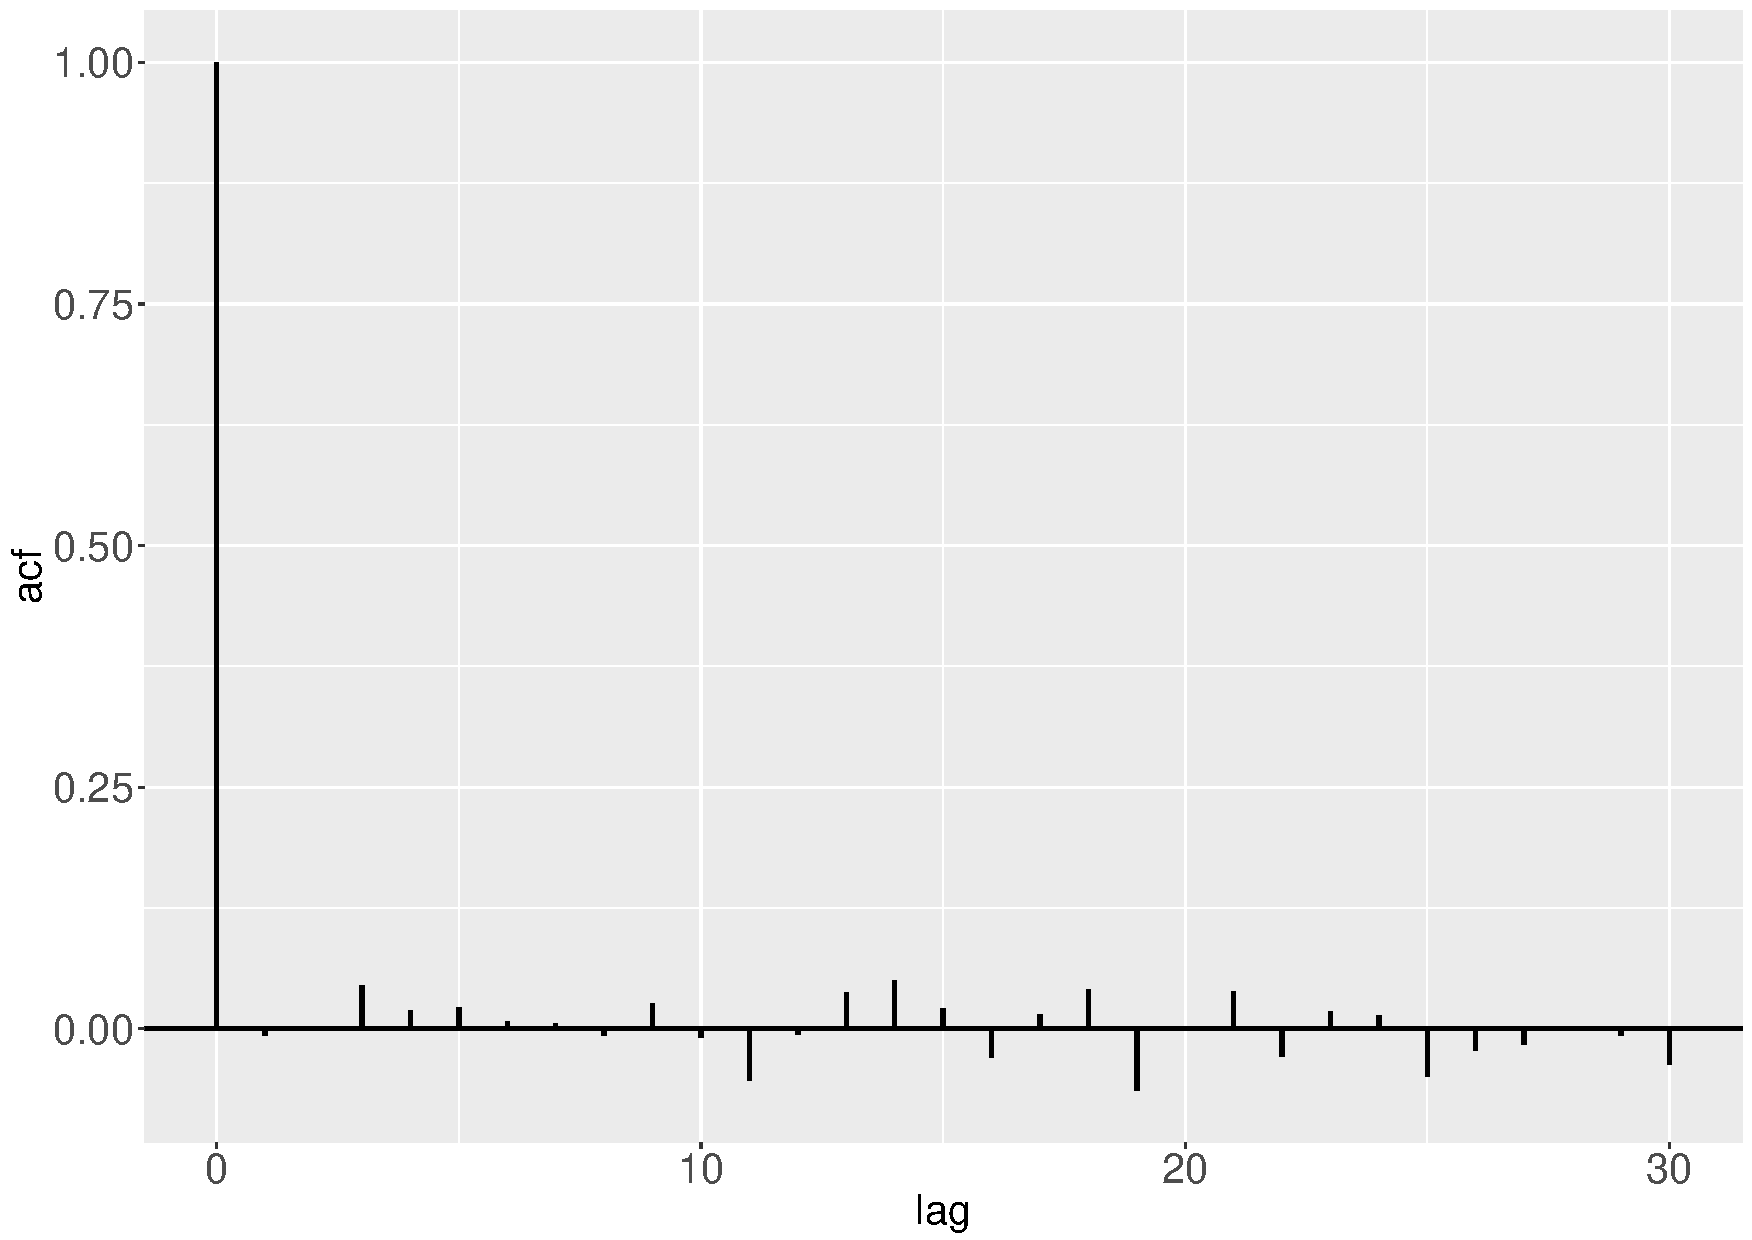
\includegraphics[width=\textwidth]{Chapters/02TractorSplineTheory/plot/ggplot/ggacfHeavi3.pdf}
    \caption{ACF of residuals from \textit{HeaviSine} with SNR at 3 }
    \end{subfigure}
    \begin{subfigure}{0.45\textwidth}
    \centering
    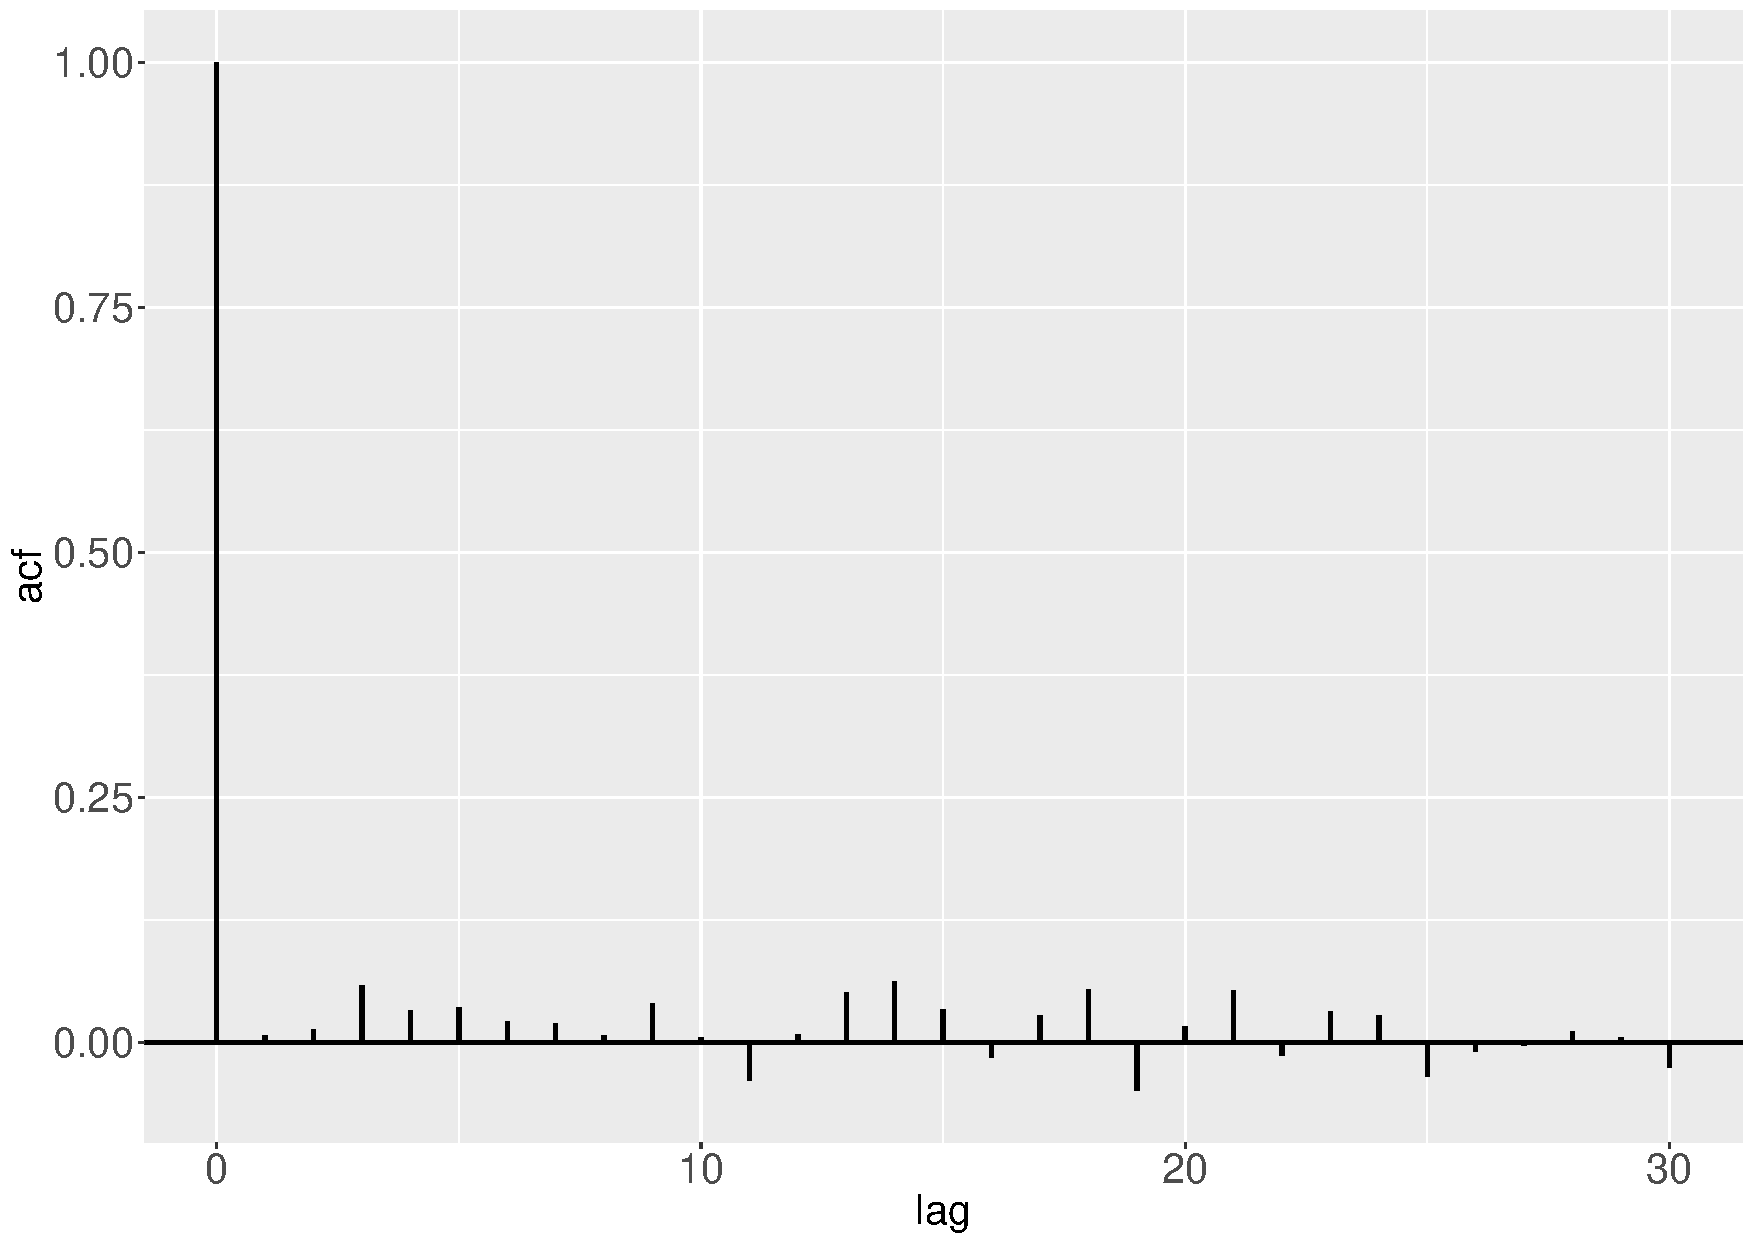
\includegraphics[width=\textwidth]{Chapters/02TractorSplineTheory/plot/ggplot/ggacfDoppler3.pdf}
    \caption{ACF of residuals from \textit{Doppler} with SNR at 3 }
    \end{subfigure}
\caption{ACF of residuals at SNR level of 3.}\label{tractorsplineSNR3acf}
 \end{figure}

\begin{figure}[!ht]
    \centering
    \begin{subfigure}{\textwidth}
    \centering
    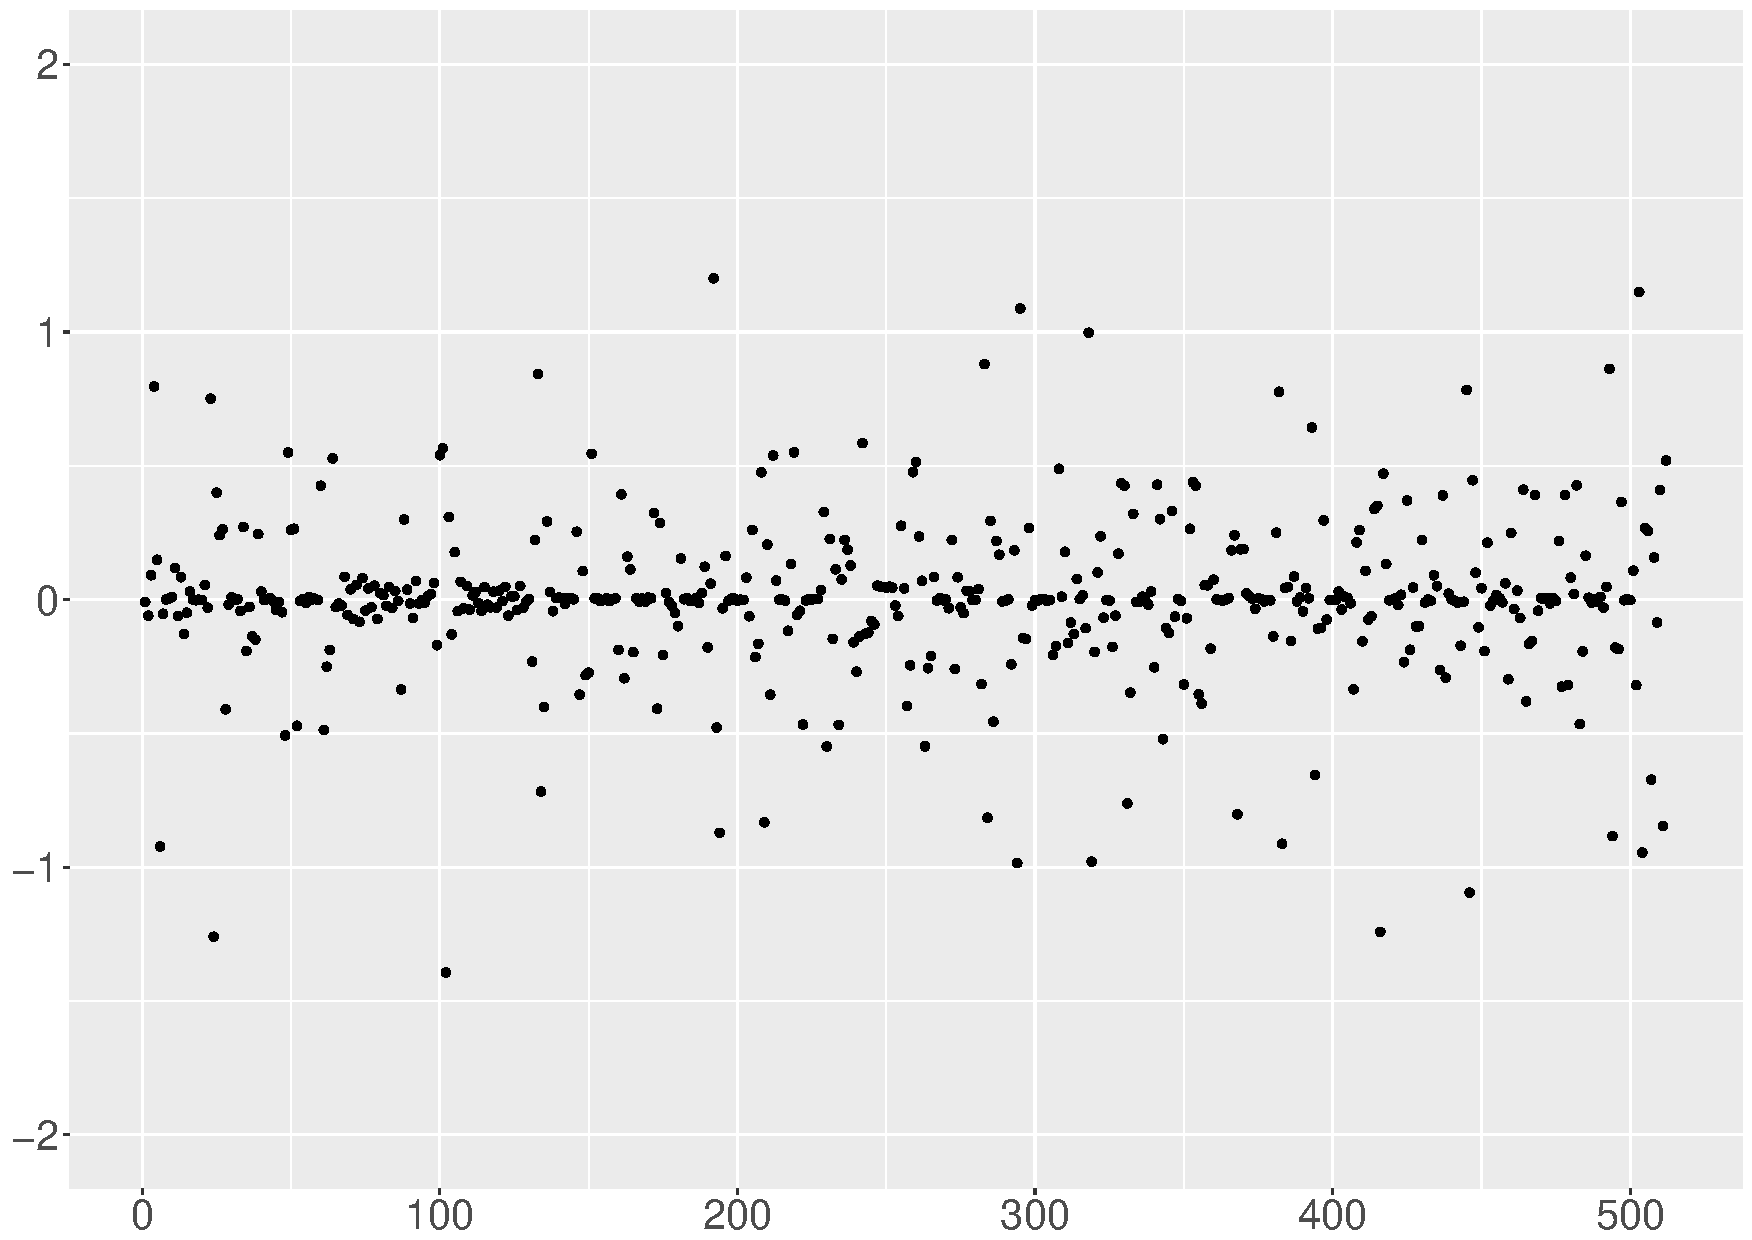
\includegraphics[width=0.45\linewidth]{Chapters/02TractorSplineTheory/plot/ggplot/ggRealdataXYResidualsXpoints.pdf}
    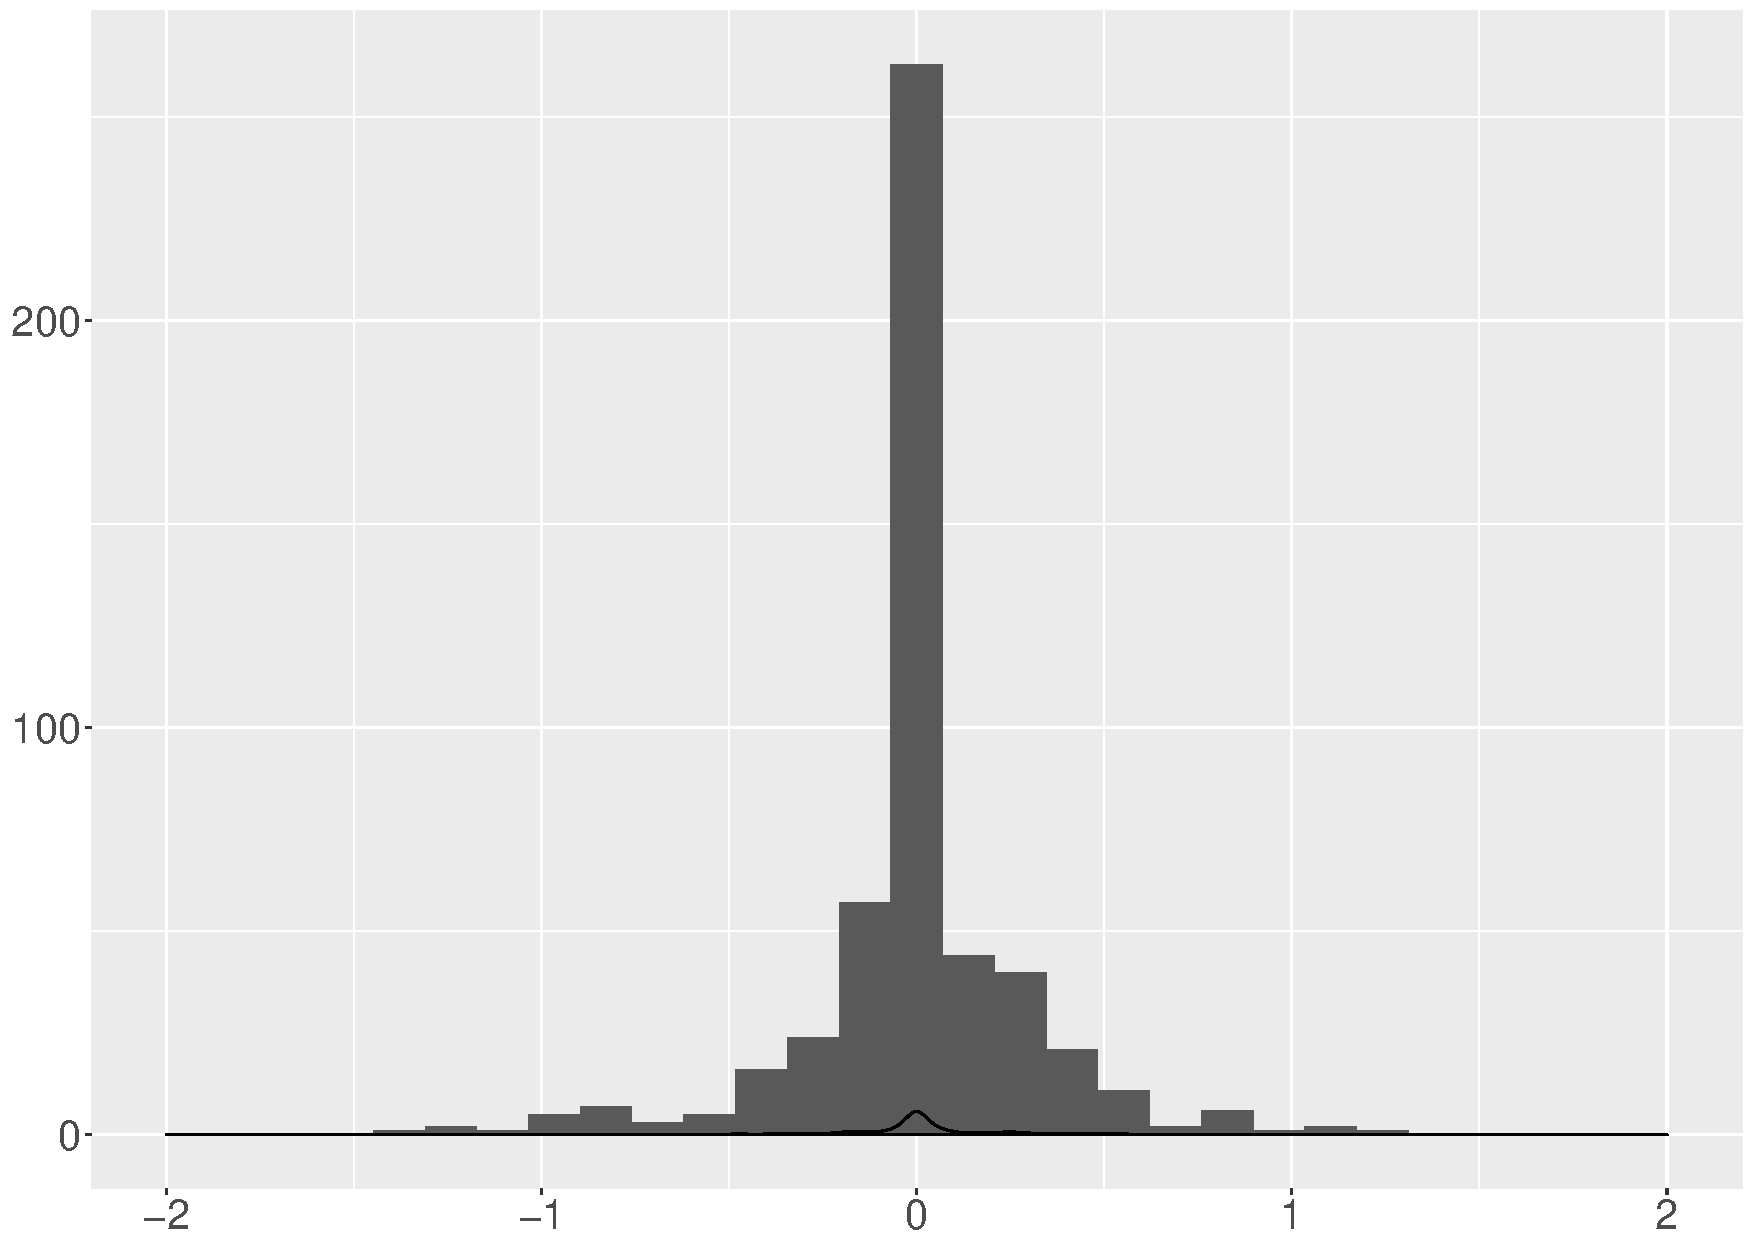
\includegraphics[width=0.45\linewidth]{Chapters/02TractorSplineTheory/plot/ggplot/ggRealdataXYResidualsXhist.pdf}
    \caption{residuals of $x$ }
    \end{subfigure}
    \begin{subfigure}{\textwidth}
    \centering
    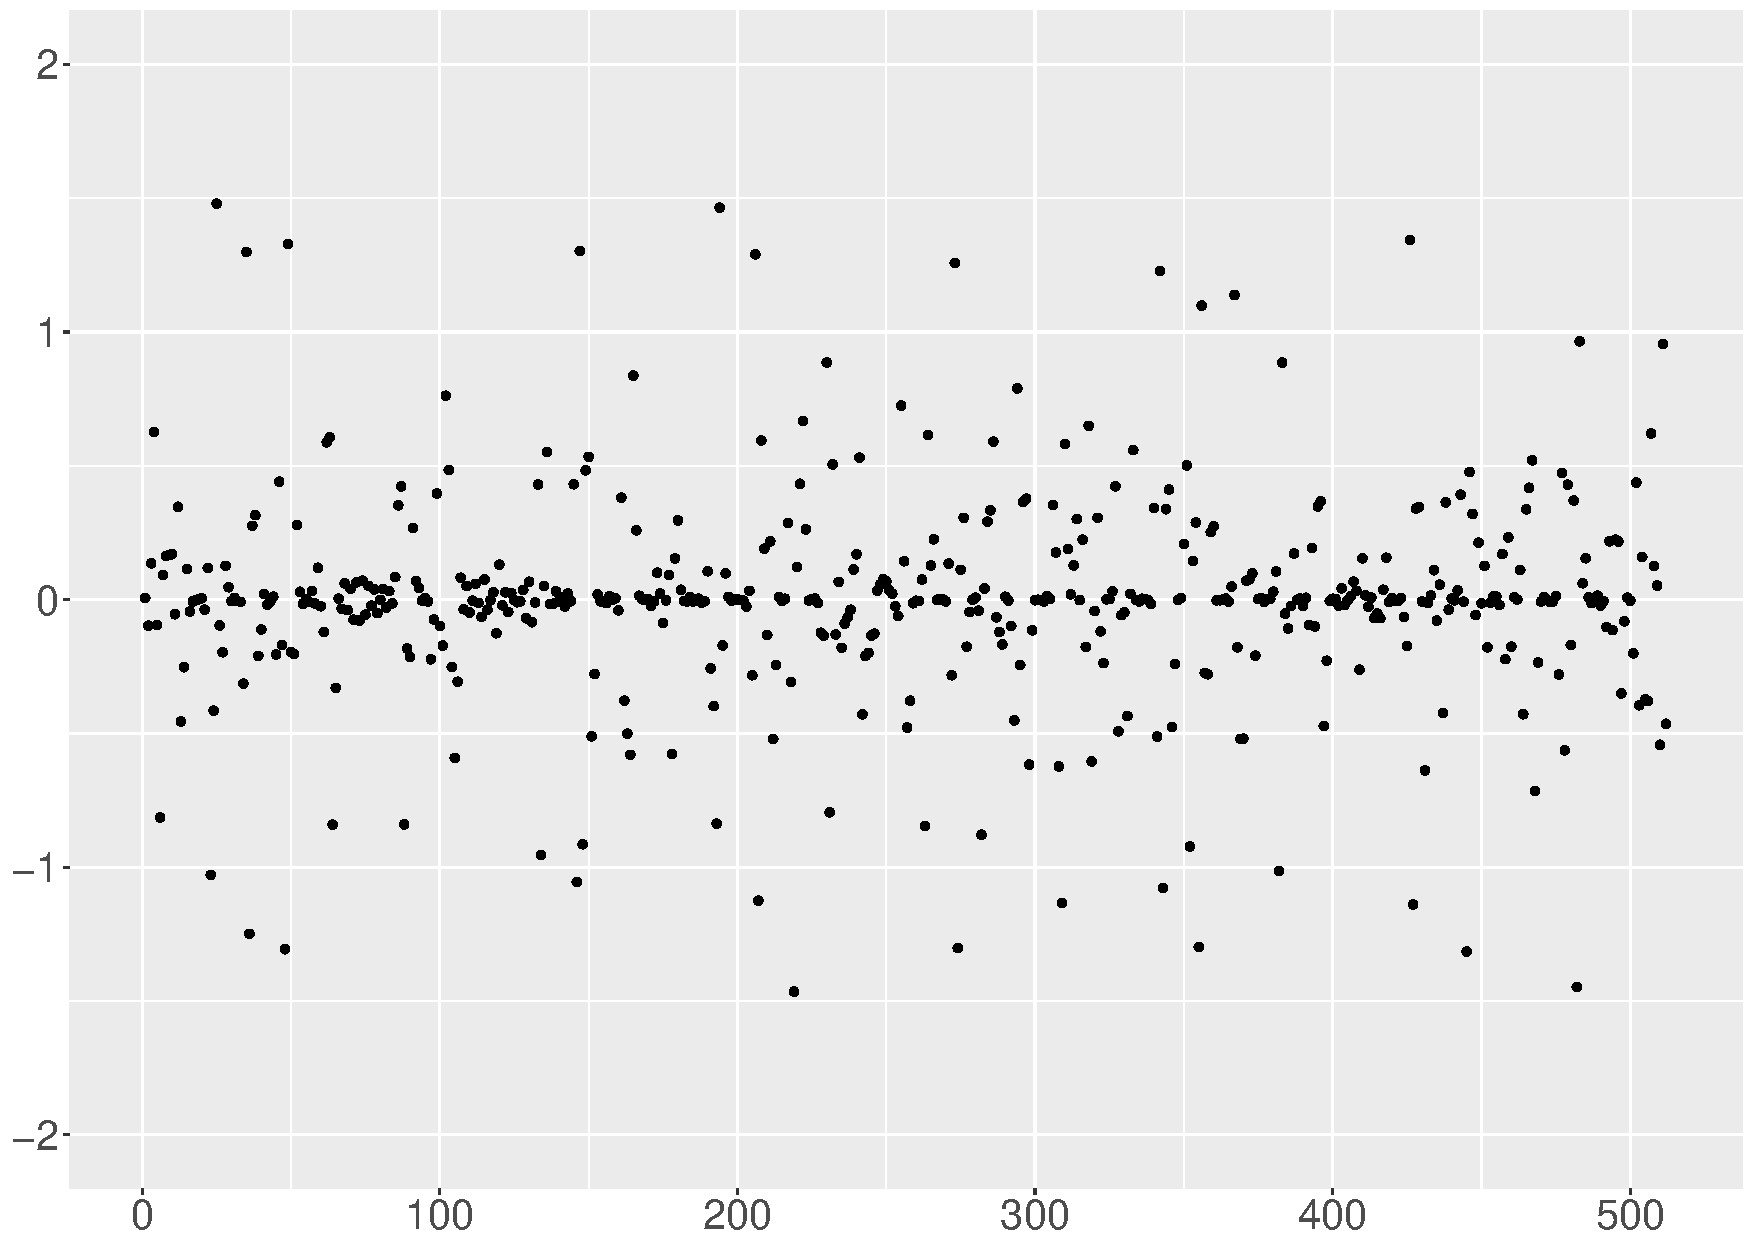
\includegraphics[width=0.45\linewidth]{Chapters/02TractorSplineTheory/plot/ggplot/ggRealdataXYResidualsYpoints.pdf}
    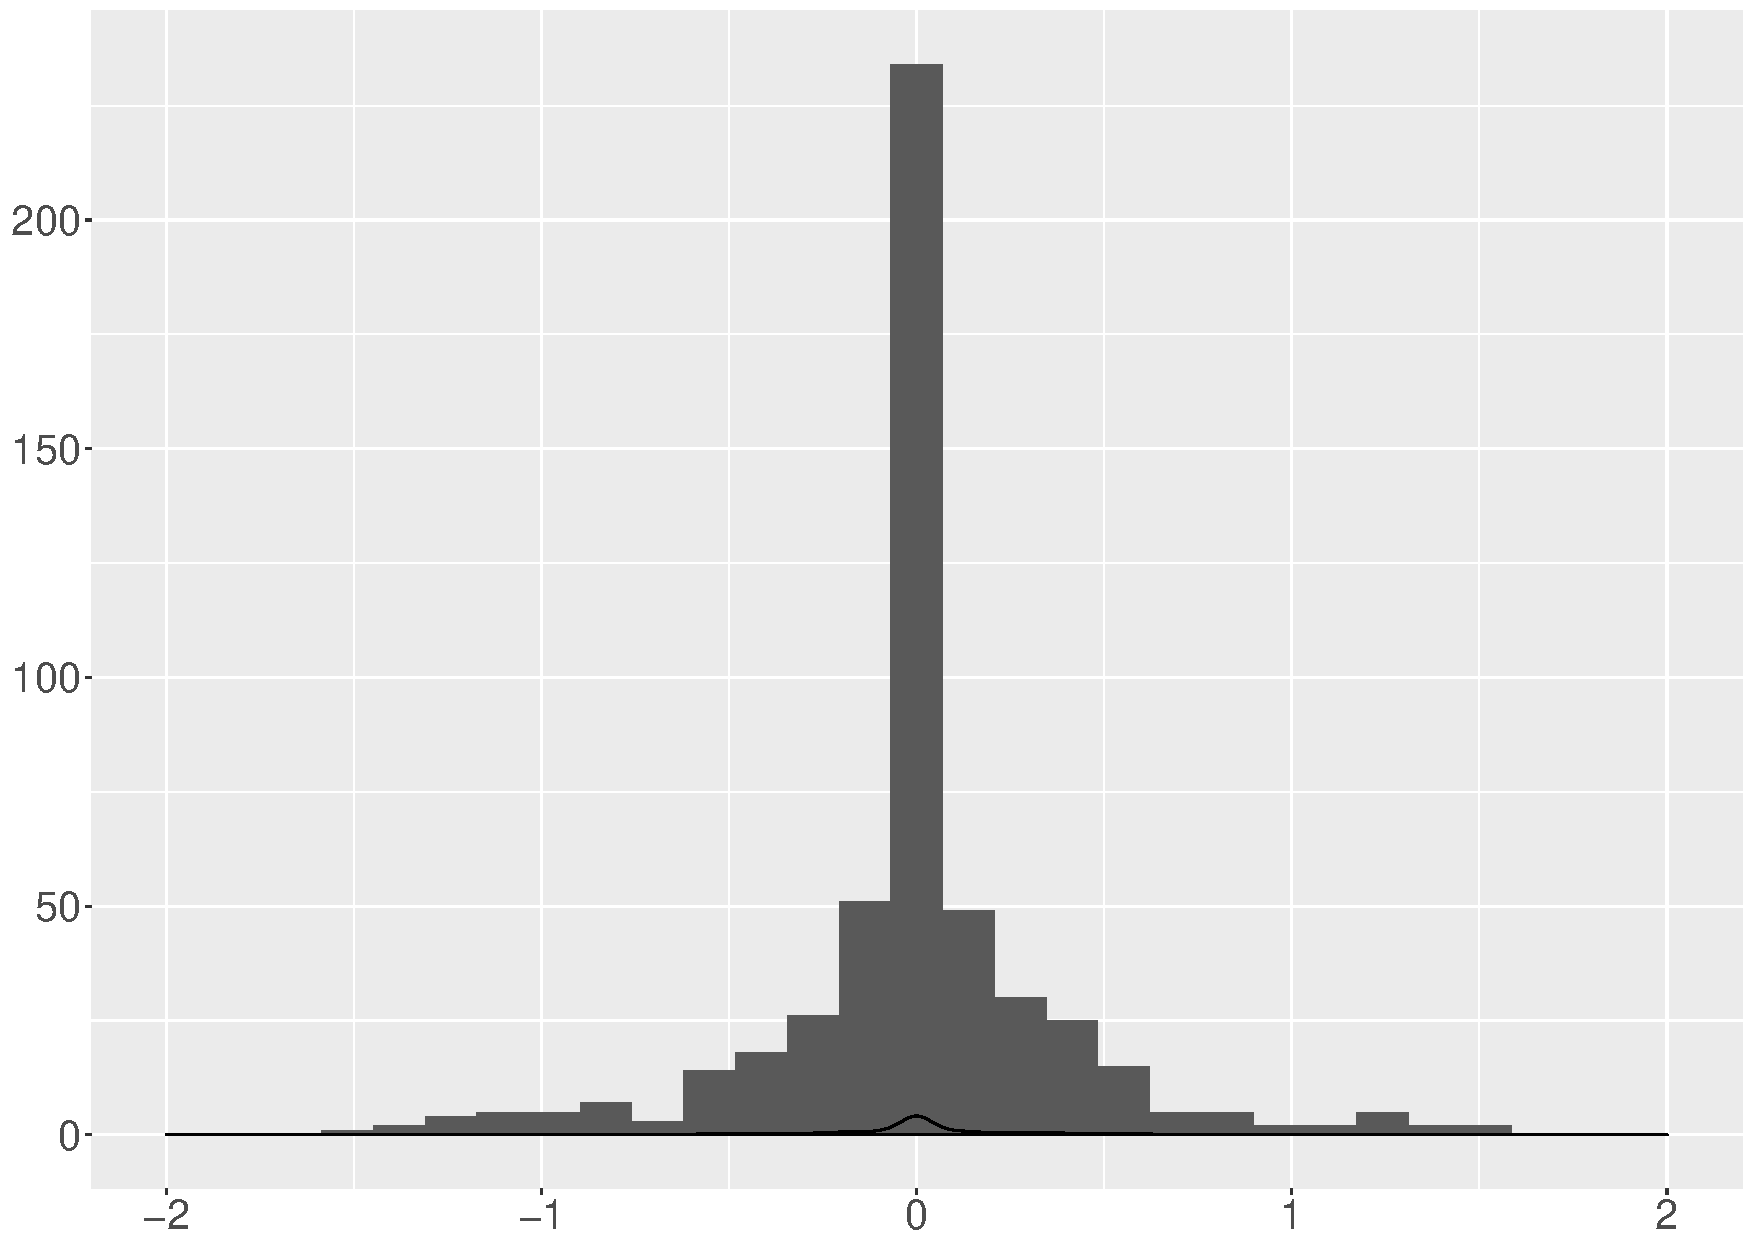
\includegraphics[width=0.45\linewidth]{Chapters/02TractorSplineTheory/plot/ggplot/ggRealdataXYResidualsYhist.pdf}
    \caption{residuals of $y$ }
    \end{subfigure}
\caption{Residuals of 2-dimensional real data reconstruction }\label{tractorsplineResidualsRealdata}
 \end{figure}

